%grand scheme
\documentclass[12pt]{article}
\usepackage{amsmath,cite}
\usepackage{graphicx}
\usepackage{courier}
\usepackage{authblk} 
\usepackage[ margin=1.5in]{geometry}
\usepackage{listings}
\usepackage{color}
\usepackage{verbatim}
\usepackage{fancyhdr}
 
\pagestyle{fancy}
\lhead{Problem Statement}
\rhead{ }

\newcommand{\figref}[1]{\figurename~\ref{#1}}
%----------------------------------------------------------------------------
%----------------------------------------------------------------------------
\renewcommand\Authfont{\small}
\renewcommand\Affilfont{\itshape\footnotesize}
%----------------------------------------------------------------------------

%----------------------------------------------------------------------------

%title
% ------
\title{Speech Prosody Mining and the Unsupervised Learning of Mandarin Tones}

\author{Shuo Zhang}
\affil{Department of Linguistics, Georgetown University}
\date{ }




\begin{document}



\maketitle
\tableofcontents

\begin{comment}
contents

1. Introduction
2. Research Questions
3. How important is tone recognition?
4. Why is tone learning hard?
5. Supervised learning of Mandarin tones
6. Unsupervised learning of Mandarin tones
7. Prosody based dialect detection via unsupervised learning
8. Chapter outlines





\end{comment}


%abstract
\pagebreak
\begin{abstract}
Tone recognition is an important and difficult task in Mandarin speech recognition that current commercial systems largely leave out. From an information theoretic point of view, tones carry at least as much as information as vowels. Recent years have seen increasing interests in the tone recognition research from the machine learning community, most of which aimed at building robust supervised machine learning system with improved accuracy, while limited effort has been made in unsupervised approaches. In my doctoral thesis work, I explore the speech prosody mining and unsupervised learning of Mandarin tones. In this document, I define the problem of unsupervised learning of Mandarin tone and identify the major challenges in tone recognition by both supervised and unsupervised learning systems. I then outline the main relevant topical areas of research and review the previous works on each of those areas while expanding the exploration of the research questions. Finally, I briefly describe the tentative plans for my thesis work and outline the intended chapters.
\end{abstract}


\section{Introduction}

Tone recognition is an important and difficult task in Mandarin speech recognition that current commercial systems largely leave out [7]. From an information theoretic point of view, tones carry at least as much as information as vowels [1]. Recent years have seen increasing interests in the tone recognition research from the machine learning community [2-5]. 

Several major challenges make tone recognition in spontaneous speech a difficult task. First, although traditionally being the single most important cue of tone recognition, the F0 contour based features alone are often considered to be insufficient, and must be coupled with other types of features such as intensity, voice quality, etc [1]. However, the improvement by incorporating these features is usually small. Second, it has been shown that the distortion of F0 contours from the canonical templates of tone categories (i.e., �the surface tone contour variability problem�) mainly comes from two sources : (1) local context, i.e., coarticulation caused by the adjacent tone environments of the current syllable, due to the physiological and phonological constraints; (2) Higher level �broad� range context, or sometimes known as �expressive functions�[6] outside of prosodic domain, such as focus, sentence modality (e.g., question vs. declaration), and sentence length. Therefore, how to identify and exploit this context information in order to restore the underlying tone target can be crucial to substantial improvement in utilizing F0 based features in tone recognition. Third, to this date, most systems of tone recognition employ supervised learning, which relies on the high cost of manually annotating and labeling a large amount of audio data.   

There has been limited effort on the unsupervised and semi-supervised learning of tones. [7,8] explored the clustering of Mandarin tones and English pitch accent using spectral clustering with both F0 and intensity features. The result is in general worse but in many cases comparable to the best supervised algorithms. However, many aspects of this unsupervised learning task can be further investigated, including (but not limit to) the most effective use of feature representation, distance measures, and clustering algorithms.  

In the meantime, unsupervised learning of tones using time-series mining techniques has shown great potential for improving the efficiency and accuracy of this task. [9] showed that by viewing tone F0 contours as a collection of time series, we�re able to employ techniques from time-series mining to speed up the computation of distance measures as well as requiring less storage space. The Symbolic Aggregate approXimation (SAX) representation of time series allows for efficient computation based on string based algorithms, while achieving better clustering accuracy on a read speech data set than using numeric representation with Euclidean distance (and comparable with numeric feature using Dynamic Time Warping distance measure, and the First Derivative (D1) feature with Euclidean distance). However, this approach is yet to be evaluated on a comparable data set as [7,8], as well as spontaneous speech data sets.  


\section{Research Questions}
This Problem Statement is based on the following goals and research questions of my thesis project.  

This project has two main goals:

(1) In \textbf{speech prosody mining}, use time-series mining and pattern discovery to better understand the F0-contour prosodic patterns in a corpus of spontaneous speech and the sources of variation for F0 tone variation. This part is carried out with annotated metadata of syllable boundaries, tones, and other non-acoustic information.

(2)  In \textbf{unsupervised learning of tones}, use various context-dependent modeling and unsupervised learning to improve the accuracy of tone recognition. 

In this project, we focus on the problem of unsupervised learning of Mandarin tones with the following research questions:  

\textbf{(1) Better understanding the tone recognition problem.} Are human listeners always able to recognize tones in or out of context, based on acoustic signal alone with reasonable high accuracy? If not, from a information theory perspective, how much information does tone carry comparing to the segmental, lexical and other non-tonal contextual information in human speech understanding? (in other words, how much can Mandarin speakers understand from mono-tone Mandarin speech? This has implications on the question of how well should we expect a tone recognizer to perform based on acoustic information alone) 



\textbf{(2) Context-dependent modeling in tone recognition.} 

(2a) What can we learn about the sources of variation for tone F0 contours in a large speech corpus, by using time-series mining based pattern discovery algorithms?

(2b) How can we incorporate local context-dependent (i.e., coarticulation depending on the adjacent tone contexts) information to modify the F0 contour time series that makes the unsupervised or semi-supervised learning more effective? 

(2c) How can we incorporate broader context information (e.g., focus, modality, etc.) to improve tone recognition accuracy in an unsupervised framework?


\textbf{(3) Features.} Using these techniques, can we obtain comparable or better performance using 
F0 contour based features alone?  

\textbf{(4) Unsupervised learning.} How can we combine F0 based features with other types of features (e.g., spectral) to improve the performance in an unsupervised or semi-supervised framework?   

\begin{comment}
Upon investigating each of these questions, we then explore the potential applications of this framework in the unsupervised learning of prosody-based dialect detection based. In this sample task, in a collection of speech segments, each segment is a \textit{m}-minute speech recording spoken in one of n Mandarin Chinese dialects. The final goal is to cluster the prosody profiles of the segments so that each cluster reveals a type of dialect. Operationally, we break the problem of prosody profile clustering into an unsupervised tone recognition task (investigated in the previous chapters of the thesis), and we use the result from that task to then do the dialect prosody clustering on a higher level.    

\end{comment}


\section{How important is tone recognition?}
Until very recently, the state-of-the-art speech recognition of tone languages typically discard tone information altogether. There has been many discussions on why this is so [ ], which is mainly attributed to the high error rate of tone recognition that supersedes the benefit of including tone information. Recent development in tone recognition, however, reveals the importance of tone information in speech recognition from a information theoretic point of view. In [Surendran 2004], the functional load of tones is found to be at least as high as vowels while lower than the consonants. Here, the functional load of tones (FL) is defined as the information we lose if the phonological system loses the contrast posed by tones: 

 %%%%%%%%%%%%%%%%%%%%%%%% E Q U A T I O N %%%%%%%%%%%%%%%%%%%%%
 
\begin{equation}
FL (tone) = \frac {H(M_u)-H(M_u^{-tone})} {H(M_u)}
\end{equation}
%%%%%%%%%%%%%%%%%%%%%%%%%%%%%%%%%%%%%%%%%%%%%%%%%%%%%%%%%%%%%%%%%%%%



where $M_u$ is a sequence of units of type U in Mandarin, U being either a a syllable or word in the entropy function H(.) calculation, $M_u^{-tone}$ refers to such a sequence without tone contrast, and H(.) is the standard entropy function of the system (i.e., a well defined \textit{language}). FL is defined as the functional load of tone. Intuitively, it characterizes how much information the system lose if the tone contrast is lost, therefore how important is a contrast within a phonological system. Table \ref{table:models} shows the functional load of tones versus other segmental contrast in Mandarin. 

%%results
\begin{table}[h]
 \caption{Functional Load of tones vs other contrasts in Mandarin}
 \label{table:models}
 \begin{center}
 \begin{tabular}{c || c | c}
  \hline
  x & $FL_{syll}$(x) & $FL_{word}$(x) \\
  \hline
  Consonants & 0.235 & 0.081\\
  Tones & 0.108 & 0.021\\
  Vowels & 0.091 & 0.022\\
  Stops & 0.029 & 0.006\\
  Fricatives & 0.021 & 0.005\\
  \hline
  Place&0.065&0.014\\
  Manner&0.034&0.006\\
  Aspiration&0.002&0.0003\\
  \hline
 \end{tabular}
\end{center}

\end{table}



This analysis captures the importance of tones in Mandarin speech recognition systems. However, it should also be interpreted carefully. First, it has the implicit assumption of taking a pure phonological point of view while ignoring all other information that can be used to distinguish words and syllables such as n-grams language models, which uses non-acoustic information during HMM based speech recognition. 

Second, on the other hand, it also calls for an analysis of how important tone is for Mandarin speech recognition in humans. It is often an implicit assumption in tone recognition literature that humans are always able to perform with reasonably high accuracy in tone recognition even when contextual tonal, segmental, and other information are unavailable. However, speech experiments have revealed that native Mandarin speakers perform below chance in isolated syllable tone recognition when additional information usually available in speech is removed [ ], depending on the specific experimental conditions. This is also supported by additional experimental evidence that humans are able to perform with greater than 90\% accuracy in speech recognition with tone information removed in Mandarin (i.e., monotone F0 is imposed synthetically)[ ]. 

Therefore, it is also worthwhile to investigate from an information theory point of view just how important is tone to Mandarin word recognition in human speakers (which from the above discussion, would reveal that it is much less important than [Surendran 2004] have suggested). The implication of such an analysis would be that, we cannot expect a machine to perform perfectly on isolated syllable tone recognition (or context-independent) when humans cannot do it in the first place. Meanwhile, it suggests the importance to develop context-dependent tone recognition algorithms that also uses contextual information beyond the information present in the acoustic signal of isolated syllables.

%include more on the Kaifu Lee paper of how can tone help.














%%%%%%%%%%%%%%%%%%%%%%% Why SO Hard?


\section{Why is tone learning hard?}
In the canonical forms of Mandarin tone system, four tone categories are present: high-level (High tone), rising (Rising tone), low-dipping (Low tone) and falling (Falling tone). Following convention, these are also referred to as tone 1, 2, 3, and 4 in this paper. \figref{fig:4tones-levow} shows the canonical contours of four Mandarin tones. In running speech, however, the contour shapes often become much distorted from canonical shapes, making it difficult to identify correct tone categories. Therefore, the challenge of tone recognition is to identify sources of variability, and exploit these knowledge to restore the underlying tone category. In continuous speech, there are many local and broader factors that play a role in producing the final tone contour shapes. These factors are usually rather convoluted and confounded and is therefore hard to identify. It requires carefully designed control experiments to reveal the effect and function of each contributing factor. 

As an example, \figref{fig:qvss} shows how a tone-controlled production experiment reveals variability of tone contour shapes in statement vs. question sentences with varying focus position [data from Liu et al 2006] . Looking at this simple example, which is far less complex than real spontaneous speech data, gives us much clue to why is tone learning hard. First, we can see clearly that even though this is all Rising tone, most tones in this sentence have a rather flat shape, resembling the High tone. This is contrasted with \figref{fig:allhigh}, where a sentence is spoken with all high tones. Second, the variability of the tone shape is dependent on the sentence focus and modality conditions. These must also be taken into account in tone recognition with real data, where this type of uniform tone combination is highly unlikely. 

In this section we discuss previous works on the sources of variability from both speech production and prosodic modeling perspective.


%%%%%%%%%%%%%%%%%%%%%%a figure
\begin{figure}
 \centerline{\framebox{
 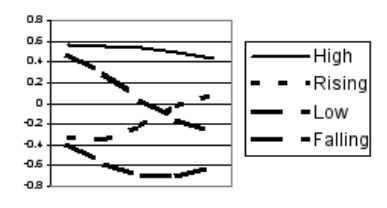
\includegraphics[scale=0.5]{4tone-levow.png}}}
 \caption{Mandarin 4 tones canonical contour shapes (adapted from [Levow 2006])}
 \label{fig:4tones-levow}
\end{figure}

%%%%%%%%%%%%%%%%%%%%a figure
\begin{figure}
 \centerline{\framebox{
 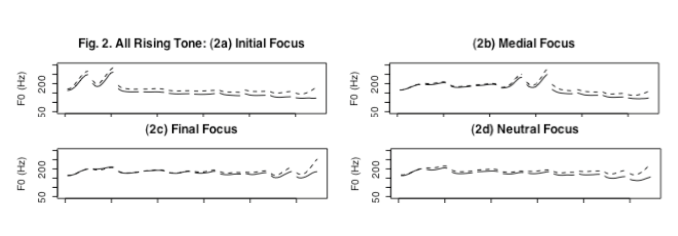
\includegraphics[scale=0.5]{allrise.png}}}
 \caption{Experimentally controlled production of all Rising tones in statement vs question sentences with varying focus position (adapted from [Liu et al 2006])}
 \label{fig:qvss}
\end{figure}


%%%%%%%%%%%%%%%%%%%%a figure
\begin{figure}
 \centerline{\framebox{
 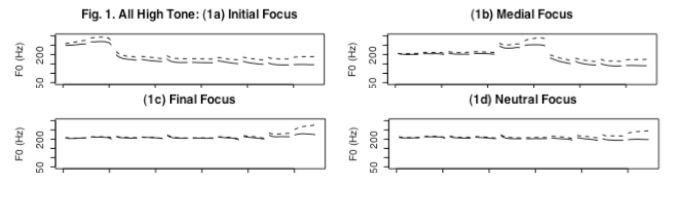
\includegraphics[scale=0.5]{allhigh.png}}}
 \caption{Experimentally controlled production of all High tones in statement vs question sentences with varying focus position (adapted from [Liu et al 2006])}
 \label{fig:allhigh}
\end{figure}



\subsection{Sources of variability: Evidence from speech perception and production}
[Gauthier et al 2007] identified two major sources for the extensive overlap between the tone contour shapes in running speech. The first is the difference in the pitch range of individual speakers and the second is the variability introduced by tonal context in connected speech [Shen 1990, Xu 1997]. In tone recognition literature, the speaker difference is usually removed by normalization. The tonal context, as mentioned above, is where the majority of the research effort has been devoted in identifying and isolating sources of variability. 

Recent works from speech production and perception experiments have made substantial progress on identifying sources of variability in tone production by carrying out experiments with carefully controlled conditions and designed data set[ ]. These experimental works also became important references for the tone recognition research community, as it is important to also exploit these knowledge in the machine learning of tones and recover underlying tone target. These are referred to as context-dependent (CI) models. 

It is generally assumed that the prosodic contours in Mandarin is shaped by at least two different levels of factors: tones, which work at the syllable level, and intonation, which works at a higher level (phrase, sentence, etc). As mentioned above, the great difficulty to isolate these layers of factors from the observed prosodic contour in speech data calls for carefully designed production studies that vary one set of factors while keeping the other set fixed. Recent works of such nature have identified the two levels of sources for tone variability in continuous speech production: First, a \textit{local context} refers to the distortion to tones from its canonical shapes due to the co-articulation with adjacent tones. Second, a \textit{broad context} refers to the further modification of tones on the intonation level of a larger prosodic unit than syllable. Examples of broad context including the topic, focus, and modality of a sentence. Often these broad contexts originate from domains outside of the phonological and articulatory constraints of speech production, and is motivated by communicative functions in the syntactic, semantic and pragmatic domain [ ]. The next two sections review works on both the local and broader context in tone production.




%does everything fit into local and broad context?
\subsubsection{Local context}
The local context of tone production is concerned with the behavior of tone contour F0 trajectories with regard to its immediate environment, i.e., adjacent syllables. Experiments were conducted with two principles in mind: first, to examine the effect of neighboring tones, speech production tasks are designed to reflect all different combinations of tones as target words. Second, to minimize the effect of higher level intonation, participants are asked to read the target words embedded in carrier sentences with careful speech with neutral focus. Several important results emerge from these studies of the local context. 

(1) \textbf{Local "conflicting" context distorts tone contour shapes in incompatible environments.} [Xu 1994] studied how the amount of deviation of a tone from its canonical form due to coarticulation varied depending on the nature of the tonal context. By grouping tone environments into "compatible" vs "conflicting" contexts, it was observed that in a context where adjacent tonal values agree (a "compatible" context, such as when the High tone "HH" ending with "H" is followed by a High-Falling tone "HL" beginning also with "H")\footnote{The "H"(High),"L"(Low) refers to phonological compositional representation of tones, where for example, a rising tone is represented as "LH" with two pitch targets: low and high. }, the deviation was relatively small. In a context where adjacent tonal values disagree (a "conflicting" context, such as when the said High tone is followed by a Low-Rising tone "LH" starting with "L"), the deviation was much greater, sometimes even to the extent of changing the direction of a dynamic tone.\footnote{The authors refer to tones with moving targets as "dynamic tone" (such as a low-rising tone), vs. static tone, where the tone has stable pitch targets (such as a high tone). } 

The author also examined the perception of co-articulated tones when tones are presented out of context in isolation. The results suggest that identification of tones in the compatible context was highly accurate with or without the original tonal context. Tonal identification for the conflicting context remained accurate only when the tones were presented with the original tonal context. Without the original context, i.e., in isolation, correct tone identification dropped below chance. As discussed above, this result provides important counter-evidence to the "myth" in tone recognition literature that human listeners are always able to recognize tones with high accuracy, even when they're distorted and in isolation. 





(2) \textbf{Carry-over effects is greater than anticipatory effects in tone co-articulation.} [Xu 1997] examines acoustic variations of tones in Mandarin under the influence of different tonal contexts. In particular, variations in the four Mandarin tones due to anticipatory and carry-over effects are analyzed by examining the time course of f0 contours of bi-tonal sequences. Using balanced nonsense sequences produced in different carriers with balanced tonal structures, this study establishes a baseline for local contextual tonal variation in Mandarin. It is found that anticipatory and carry-over tonal influences differ both in magnitude and in nature. Carry-over effects are mostly assimilatory: the starting f0 of a tone is assimilated to the offset value of a previous tone. Anticipatory effects, on the other hand, are mostly dissimilatory: a low onset value of a tone raises the maximum f0 value of a preceding tone. While the magnitude of the carry-over effect is large, anticipatory effects are relatively small. This conclusion has been cited many times subsequently by tone recognition researchers, whose own data analysis also showed support for this asymmetry over and over again[ ]. There are also many machine learning approaches that take this effect into consideration in tone modeling.  

%need more comments
(3) \textbf{Physiological constraints of tone co-articulation. } [Xu and Sun 2002] studied the maximum speed of pitch change in human speech production, which contributes to the understanding of the underlying mechanism for tone co-articulation and its implication for tone modeling. An experimental paradigm was adopted in which subjects (native speakers of English and Mandarin) produced rapid successions of pitch shifts by imitating synthesized model pitch undulation patterns. The speed of pitch change was measured both in terms of response time and excursion time�time needed to complete the entire pitch shift. Results show that excursion time is nearly twice as long as response time. Also, it is found that the maximum speed of pitch change varies quite linearly with excursion size, and that it is different for pitch rises and falls. Comparisons of present data with data on speed of pitch change from studies of real speech found them to be largely comparable. This suggests that the maximum speed of pitch change is often approached in speech, and that the role of physiological constraints in determining the shape and alignment of F0 contours in speech is probably greater than has been appreciated. 

(4) \textbf{F0 peak delay.} Fundamental frequency (F0) peak delay refers to the phenomenon that an F0 peak sometimes occurs after the syllable it is associated with either lexically or prosodically. Previous studies suggested that peak delay was only found in Rising tones in Mandarin [  ]. [Xu 2001] investigated peak delay and its relationship with tone, tonal context, and speech rate. Analysis of F0 contours and peak alignment revealed that at normal speech rate, peak delay occurred regularly in both the R and weakened H tones but only occasionally in the H tone; at slow speech rate, peak delay continued to occur regularly in the R tone but only occasionally in weakened H and rarely in the H tone; at fast speech rate, peak delay occurred not only regularly in the R and weakened H tones, but also frequently in the H tone. Results of F0 contour alignment analysis indicate that peak delay occurs when there is a sharp F0 rise near the end of a syllable, regardless of the cause of the rise. The author concluded that much of the variability in the shape and alignment of F0 contours in Mandarin is attributable to the interaction of underlying pitch targets with tonal contexts and articulatory constraints, rather than due to actual misalignment between underlying pitch units and segmental units.





%To me, as interesting as this paper is, the biggest implication of the results is the question I have been asking for a long time: can human listeners correctly identify the tones independently in isolation without using any other information, such as lexical and semantic information in the context and in the segments? The answer in no. The further implication of this answer is simply that we cannot expect machines to do this in continuous recognition of tones in an independent manner. This is a fundamental conundrum of this task. We should perhaps try to establish an upper limit, given human performance, and try to perform an experiment to determine this limit. Humans, when performing this task in a regular context, has the advantage of incorporating other information in lexical statistical properties of n-grams and of semantic, syntactic, etc., information, that in speech recognition is not always the easiest to acquire with high accuracy.













\subsubsection{Broad context}
In this section we review previous works regarding the effect of broad context on tones in speech production and perception. 


(1)\textbf{Focus in the temporal domain. } It is well known that focus affects the pitch of what is being
focused. More importantly, [Xu et al 2004] showed that focus also extensively affects the pitch ranges of non-focused regions in a sentence, suggesting a wide effect of focus on the temporal domain. Results from this study show that in a declarative sentence, focus is realized not only by expanding the pitch range of the focused item, but also by compressing the pitch range of post-focus items, and possibly requiring that the pitch range of pre-focus items remain neutral. The authors proposed that the domain of a single, narrow focus consists of three temporal zones (pre-focus, on-focus, post-focus), with distinct pitch range adjustment for each. This proposal has received positive support when it was later applied to a machine learning model that improves tone recognition accuracy by incorporating focus information[Surendran 2005]. [Liu et al 2006] also used focus as an effective input feature to a decision-tree based classifier to predict the modality of a sentence from the prosodic domain (question vs. statement).

%this is important, include the detailed description
In [Xu 1999] , the author further examined how lexical tone and focus contribute to the formation and alignment of F0 contours using short Mandarin sentences consisted of five syllables with varying tones on the middle three syllables. The sentences were produced with four different focus patterns: focus on the first, second, or last word, or with no narrow focus. The results indicate that while the lexical tone of a syllable is the most important determining factor for the local F0 contour of the syllable, focus extensively modulates the global shape of the F0 curve, which in turn affects the height and shape of local contours. Moreover, despite extensive variations in shape and height, the F0 contour of a tone remains closely aligned with the associated syllable.


(2)\textbf{Long-term F0 variations.} Many tone recognition algorithms incorporate features that encode the relative pitch heights of the tones [ ], in conjunction with the features that encodes the contour shapes. However, the pitch heights of tones in longer temporal units of spontaneous speech (e.g., a sentence) must be normalized not only based on individual speaker differences, but also to compensate for the long-term F0 pitch variations due to factors such as down-drift and other pragmatic functions such as focus and topic. 

[Wang and Xu 2011] reports an experimental investigation of the prosodic encoding of topic and focus in Mandarin by examining disyllabic subject nouns elicited in four discourse contexts. They also looked at how prosodic effects of topic and focus differ from each other and how they interact with sentence length, downstep and newness to determine sentence-initial F0 variation. Sixty short discourses were recorded with variable focus, topic level, newness, downstep, and sentence length conditions by six native speakers. The important conclusions include: 

(a) The difference between topic and focus lies in that focus both raises on-focus F0 and lowers post-focus F0, while topic raises the F0 register at the beginning of the sentence while allowing F0 to drop gradually afterwards.

(b) topic has higher pitch register in isolated and discourse-initial sentences than in non-initial sentences,

(c) longer sentences have higher sentence-initial F0 than shorter sentences, but the differences are small in magnitude and are independent of topic and focus,

(d) the effect of downstep is independent of topic and focus, but is large in magnitude and accounts for a significant amount of the F0 declination in a sentence,

(e) newness has no F0 manifestation independent of other factors, but a newly mentioned word is slightly longer than a previously mentioned word, and

(f) the effects of topic, focus, downstep and sentence length are largely cumulative.



%me: the cumulative nature of the different functions is said to support the PENTA model, which cumulatively encode and add the effects of each communicative function.










\subsection{Prosodic modeling}

Research in prosodic modeling provides evidence and often validation to the results obtained from speech production experimental works in tone variability. The goal of prosodic modeling is to analyze and synthesize speech prosody that is as natural as possible, while requiring less resources in storage, computation, and supervision. These models are often used to generate F0 contours for speech synthesis. As such, typically prosodic models are evaluated by means of its capability to (1) re-synthesize speech melodies that closely approximate the original data (training data) ; (2) predicatively synthesize / generate speech melodies of unseen data given annotated sentence and syllable conditions (i.e., input features). Most systems include an evaluation of (1) but only few aim to do (2).


%what are we most interested in in prosodic modeling?
%  representation of intonation and tone; modeling of F0 generation process

Meanwhile, on a different level, prosodic modeling is also associated with the theoretical aspect of the representation of speech intonation in the suprasegmental domain of phonology, and the underlying mechanism for the production and perception of speech prosody. While the current project is not concerned with either the generation of F0 contours for speech synthesis or the phonological and psycholinguistic theory of speech production and perception, there are a few aspects in prosodic modeling that can shed light on the machine learning of tones. Specifically, the representation of intonation is directly relevant to the choice of the type of feature vectors we use in tone recognition. Moreover, the modeling of F0 generation process can also provide clues as to how tone variability occurs in real-time spontaneous speech. 

In the next two sections, I follow the convention in speech prosodic modeling and divide the review of relevant works into two parts: phonology-based and phonetic-based models. One of the phonetic-based models of particular interest to Mandarin is the pitch Target Approximation and PENTA model [Prom-on et al 2009 ], which I will discuss separately. This model was developed specifically with Mandarin tones in mind, while it has been also generalized to be a language independent model.  
  







\begin{comment}
%In contrast to learning a representation of F0 trajectories (as exemplified by [Gauthier et al 2007] and this paper), other researchers have approached tone modeling by taking into account the phonological processing of tone production and perception. [Moren and Zsiga 2006] in their study on Thai, vary from the standard notion of associating targets to syllables, but instead propose a model of tone phonology which involves associating tone targets with the syllable moras. Building on this work and the gating experiments [Lai:08]that showed the predictive nature of tone perception, [Ramadoss 2009] proposed a Bayesian-inference based tone recognition model that predictively compute the probabilities of incoming tone signals based on past exposure to tones in Thai. Ramadoss commented that "While these maps [in [Gauthier et al 2007]] may achieve perceptually equivalent results, the predictions are different. The main point to note is that this model does not refer to the phonology of tone. The tones are encoded as strings of f0 values that are matched point-by-point with category values. Hence, according to this model, tone perception is uninformed by phonology, and is simply a matching process between incoming f0 values and a category template." In this alternative phonologically informed view, instead, with the general notion of tonal targets, production of tones can be thought of as an interpolation between the various targets, and hence perception of tones in understood as an attempt to identify these targets. Since each tone category has a specific target template, based on the tones associated to its syllable moras, categorizing tones reduces to matching the identified targets to the templates [Ramadoss 2009].
\end{comment}


%this section should be done by reading both Sun's review and Xu's prosody review, and pick what is relevant plus some comments of its utility in the present project.

%important: be concise and pick what is relevant here. 

%point of Sun: it is not that hard to fit some parameters that can generate a curve that closely resemble the original one; it is much harder to achieve the ideal goal of prosodic modeling with linguisitically meaningful parameters.


\subsubsection{Phonology-based models} \label{sec:prosodic}


%overview of phonological models
The goal of a phonological model is to study the universal organization and underlying structure of intonation. Complex intonation patterns are compressed into a set of highly succinct and abstract vocabulary with wide coverage. These (categorical) symbols are regarded as the primitive entities in representing intonation. The development of such an inventory is often based on phonetic analysis of F0 curves either from a production perspective or from a perception perspective.

%AM model
One of the dominant views on intonational phonology is the Autosegmental-Metrical (AM) model [Goldsmith 1990; Ladd 1996]. Ladd (1996) states four principles of the AM approach to intonation:Linearity of tonal structure; Distinction between pitch accent and stress; Analysis of pitch accents in terms of level tones; Local sources for global trends.

The most influential example is Pierrehumbert�s model for American English [Pierrehumbert 1980]. The original model has been extended by Beckman and Pierrehumbert [1986], and has evolved into a standard for transcribing intonation of American English - Tone and Break Indices (ToBI) [Silverman et al 1992].
The main idea of Pierrehumbert�s model, or AM approach in general [Ladd 1996], is that English intonation can be represented by two types of tones: High and Low. The model describes intonation with multiple levels. The largest prosodic unit is called intonational phrase, which can contain several intermediate phrases. A phrase is represented as a sequence of high (H) or low (L) tones. 

The tone inventory include: \textit{Pitch Accents} can be either single tones (H*, L*) or bitonal (H*+L, H+L*, L*+H, L+H*). The * symbol represents the alignment of a tone with the accented syllable. \textit{Boundary tones}, denoted by the �\%� symbol, are single High or Low tones aligned with the edges of a phrase (H\%, L\%). Thus, they indicate the onset and offset pitch of an intonational phrase, respectively. \textit{Phrase accents}, indicated by the �-� symbol, are used to represent the pitch movement between a pitch accent and a boundary tone (H-, L-).

Pierrehumbert�s model has a linear structure in describing intonation in that intonation is solely determined by a local component, which is in contrast to the superpositional approach which treats intonation resulting from the addition of several components, such as a local pitch accent and a global phrase contour. The mapping from phonology onto acoustics and physiology is a dynamic interpretative process [Pierrehumbert and Beckman 1988]. In this process, a set of phonetic realization rules are applied to convert abstract tonal representation into F0 contours by considering the metrical prominence of the syllables and the temporal alignment of the tones with the accented syllables [Pierrehumbert 1981]. This direct phonology-F0 mapping implies that a distinct layer of phonetic model is not necessary.




\subsubsection{Phonetic-based models}

%overview of phonetic models
Phonetic models use a set of continuous parameters to describe intonation patterns observable in an F0 contour (Taylor, 2000). An important goal is that the model should be capable of reconstructing F0 contours faithfully when appropriate parameters are given. However, to make it functional, a phonetic model should also be linguistically meaningful. In fact, using certain functions, such as polynomial equations, to accurately represent F0 contour is not a difficult task. What is more challenging is developing a model whose parameters are predictable from available linguistic information.


% Fujisaki model

\textbf{Fujisaki Model.} [Fujisaki et al 1983, 1988] developed an intonation model for Japanese, which has also been applied to other languages (e.g., German (Mixdorff, 2000)). The model additively superimposes a basic F0 value (Fmin), a phrase component, and an accent component, on a logarithmic scale. The control mechanisms of the two components are realized as critically damped second-order systems responding to impulse commands in the case of the phrase component, and rectangular commands in the case of the accent component. The Fujisaki model attempts to relate the functions to the human speech production apparatus. It is a typical superpositional approach in that it assumes different intonation components to be superimposed on top of each other. This is different from the AM approach described above, which is predominantly sequential. One of the critical steps towards application of the Fujisaki model is the extraction of model parameters from F0 contours. Fully automatic extraction of model parameters has been developed (Mixdorff, 2000), which would facilitate researchers working with the model on large corpora.


%qTA PENTA mention

\textbf{quantitative Target Approximation. }A pitch target approximation model for generating F0 contours in Mandarin Chinese was proposed by [Xu and Wang 1997, 2001] and quantified in [Xu et al 1999] with the quantitative Target Approximation model (qTA). In this model, the surface F0 contour is viewed as the result of asymptotic approximation to an underlying pitch target, which can be a static target ([high] or [low]) or a dynamic target ([rise] or [fall]). A pitch target is defined as the smallest unit that is articulatorily operable. The host unit of a pitch target is assumed to be the syllable (for Mandarin, at least). This model is primarily based on evidence from Mandarin, where four basic pitch targets ([high], [low],[rise] and [fall]) are associated with the lexical tones in Mandarin: H (High), L (Low), R (Rising) and F (Falling), respectively. Rather than simply simulating the surface F0 contours, this model aims at some deeper speech production mechanism, which is similar to the Fujisaki model in this regard. It also emphasizes the role of articulatory constraints in intonation modeling. Due to the relevance of the qTA model to the current project, I discuss the relevant literature in more detail in the next section.


%non-parametric phonetic models
\textbf{Non-parametric models. }Both phonological and phonetic frameworks seek to model F0 contours effectively with a set of more abstract representations. However, F0 values themselves are no doubt good indicators of high-level linguistic information[Sun 2002]. As discussed above, the goal in developing parametric models is to find a better representation of F0 contours. However, if inappropriate forms are used, the predictions can be significantly different from the original F0 contours[Sun 2002]. Therefore, some  researchers use the original F0 contours directly or F0 with some trivial modifications as the output targets. Such systems are referred to as non-parametric models [Black and Hunt 1996; Ross and Ostendorf 1999; ], and often times they can achieve very competitive results. In this thesis I also experiment with such F0 based features in time-series mining, and explore how feature representations based on F0 transformations perform effectively in clustering tasks.

%some comments on model comparison based on Sun?






%PENTA and the annotation scheme plays a crucial role
%the reason here we separate this out is also b/c PENTA is the only model developed with Mandarin tones in mind and generalized to be language independent
\subsubsection{PENTA and quantitative Target Approximation (qTA)} \label{sec:qta}
%[Prom-on et al 2009] reports the development of a quantitative target approximation qTA model for generating F0 contours of speech. The qTA model simulates the production of tone and intonation as a process of syllable-synchronized sequential target approximation [Xu 2005]. It adopts a set of biomechanical and linguistic assumptions about the mechanisms of speech production. The communicative functions directly modeled are lexical tone in Mandarin and lexical stress in English and focus in both languages. The qTA model is evaluated by extracting function-specific model parameters from natural speech via supervised learning automatic analysis by synthesis and comparing the F0 contours generated with the extracted parameters to those of natural utterances through numerical evaluation and perceptual testing. The F0 contours generated by the qTA model with the learned parameters were very close to the natural contours in terms of root mean square error, rate of human identification of tone, and focus and judgment of naturalness by human listeners. The results demonstrate that the qTA model is both an effective tool for research on tone and intonation and a potentially effective system for automatic synthesis of tone and intonation.

[Prom-on et al 2009] reports the development of a quantitative target approximation qTA model for generating F0 contours of speech. The model simulates the production of tone and intonation as a process of syllable-synchronized sequential target approximation [Xu 2005]. As a speech production model, the qTA and the associated Parallel Encoding and Target Approximation (PENTA) model has generated much debate on its architecture, representation, and predictive powers [see ]. In the current context, however, we're only interested in evaluating how good is the qTA model in terms of its capability to numerically predict speech prosody contours as well as its representation of tone targets as input features to our unsupervised learning framework. The qTA model is evaluated by extracting function-specific model parameters from natural speech via supervised learning automatic analysis by synthesis and comparing the F0 contours generated with the extracted parameters to those of natural utterances through numerical evaluation and perceptual testing. In this model, each tone is produced with a pitch target in mind, defined by a linear equation with a slope and a intercept parameters, m and b:

%%%%%%%%%%%%%%%%%%%%%%%% E Q U A T I O N %%%%%%%%%%%%%%%%%%%%%%%%%%%%%%%%equations
\begin{equation}
x(t)=mx+b
\end{equation}
%%%%%%%%%%%%%%%%%%%%%%%%%%%%%%%%%%%%%%%%%%%%%%%%%%%%%%%%%%%%%%%%%%%%

However, the realization of this target is often constrained and deviated by the characteristic factors of the human vocal folds, such as the continuity of pitch change (no sudden change in the derivatives of the curves across syllable boundary) and the limitation of the maximum speed of pitch change [Xu and Sun 02]. As a result, actual F0 contours of tones are characterized by a third-order critically damped system:

%%%%%%%%%%%% E Q U A T I O N %%%%%%%%%%%%%%%%%%%%%%%%%%%%%%%%equations
\begin{equation}
f_0(t)=x(t)+(c_1+c_2t+c_3t^2)e^\lambda t
\end{equation}
%%%%%%%%%%%%%%%%%%%%%%%%%%%%%%%%%%%%%%%%%%%%%%%%%%%%%%%%%%%%%%%%%%%%

Intuitively this can be seen as casting a noise component on top of the linear pitch target. Solving this equation, we have in total three parameters to represent a tone contour with the qTA model: slope and height of the pitch target, namely, m and b, and $\lambda$, which represents how fast the pitch change is approaching the target slope and height. \figref{fig:qta} shows a number of different combinations of the parameters to demonstrate how the actual F0 behaves in accordance with the underlying pitch targets. 





%%%%%%%%%%%%%%%%%%%%%%% F I G U R E %%%%%%%%%%%%%%%%%%%%%%%%%%%%
\begin{figure}
 \centerline{\framebox{
 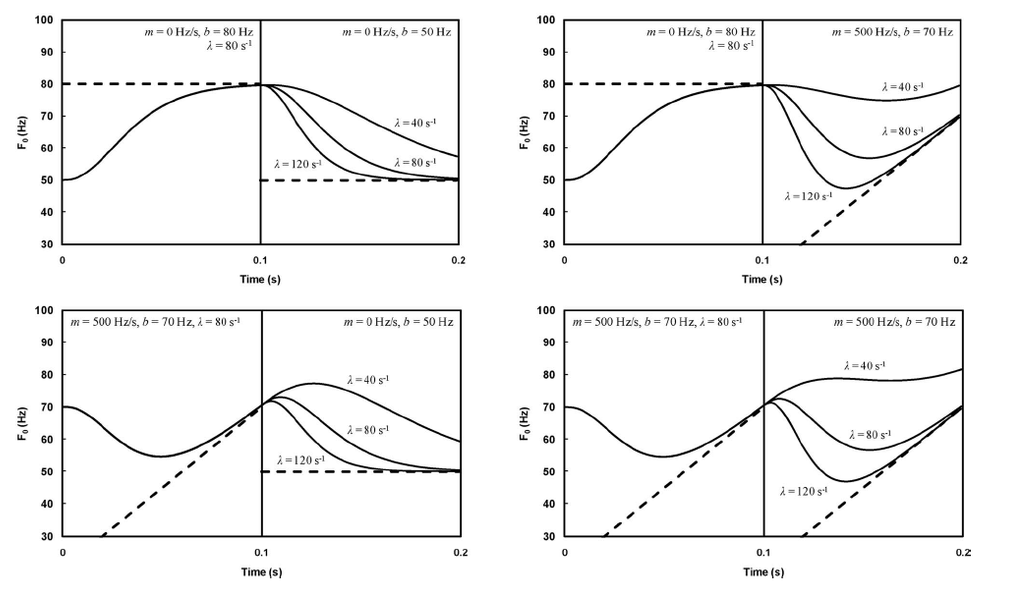
\includegraphics[scale=0.4]{qta.png}}}
 \caption{Examples of F0 contours generated by the qTA model with varying values of m, b, and $\lambda$. The dashed lines indicate the underlying pitch targets which are linear functions of m and b. The vertical lines show the syllable boundaries through which the articulatory state propagates.}
 \label{fig:qta}
\end{figure}
%%%%%%%%%%%%%%%%%%%%%%%%%%%%%%%%%%%%%%%%%%%%%%%%%%




The computational tools for extracting parameters and performing re-synthesis based on qTA model have been developed in Praat Scripting Language (PSL). In the early version of this tool (PENTATrainer1\footnote{Downloaded from http://www.homepages.ucl.ac.uk/~uclyyix/PENTAtrainer1/.}), parameter optimization is achieved by an exhaustive search through the parameter space via error minimization algorithms[Prom-on et al 2009]. The local parameter sets learned from this process are then summarized into categorical ones by averaging across individual occurrences of the same functional categories [Prom-on et al 2009]. While the synthesis results did closely approximate the original F0 contours, there are few disadvantages of this strategy. First, the estimated parameters are optimal for the local syllable but not necessarily for the functional categories. Second, the estimation of $\lambda$ is often not satisfactory because it may be stuck at a local minimum and fails to converge to global minimum[Xu and Prom-on 2014]. 


To address this problem and upgrade the qTA model to include more features reflecting function-related variability, [Xu and Prom-on 2014] developed PENTAtrainer 2 using stochastic learning from real speech data with annotations of metadata information about the sentences (referred to as layered pseudo-hierarchical functional annotation scheme, which requires the manual labeling of only the temporal domains of the functional units). More specifically, each syllable is annotated with its syllable boundaries, tone categories of the current and adjacent tones, focus / stress status, and associated sentential modality (see \figref{fig:PENTA2}. Overall, this version is characterized by its use of a functional annotation scheme, and training from the annotated data to obtain the parameter values, making it more explicitly a standard machine learning approach that encodes various types of input features. In this respect, it is unlike prosodic modeling approaches typical in previous literature. It also has the ability to predicatively generate synthesized speech melody on unseen data, given that the test data are also annotated in this set of input feature labels. The authors argue that this set of annotation is much less labor intensive than traditional frameworks [ ]. 

%discussion of dataset?


%%%%%%%%%%%%%%%%%%%%%%% F I G U R E %%%%%%%%%%%%%%%%%%%%%%%%%%%%
\begin{figure}
 \centerline{\framebox{
 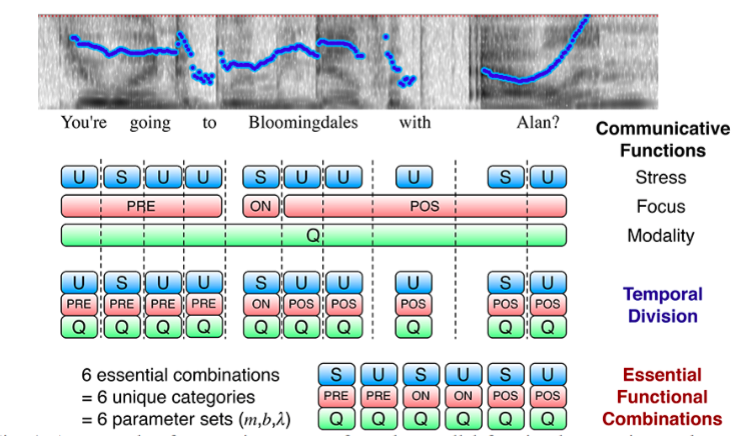
\includegraphics[scale=0.5]{penta2.png}}}
 \caption{PENTATrainer 2 annotation scheme}
 \label{fig:PENTA2}
\end{figure}
%%%%%%%%%%%%%%%%%%%%%%%%%%%%%%%%%%%%%%%%%%%%%%%%%%

%Many discussions on methodology, data set, evaluation, etc., are worth citing. There are also many excellent plots to demo the contextual variations.


%One thing that should be clear is that, even though this work demonstrates the most modern and state-of-the-art tone modeling techniques, it belongs to a different tradition than our tone recognition CS type of work, which is embedded in purely machine learning / speech recognition tradition that requires fewest resource to do tone recognition from speech signal. The Xu�s works, on the other hand, belongs to the camp of �prosodic modeling�, in which the theoretical models of the representation, re-synthesis and predicative synthesis occupy the most important place, and the syntheses essentially offer validation to the conception and theory behind it. This tradition shapes the specific ways that this work is presented, problems discussed, and algorithms outlined (and evaluated). It is good to recognize the different traditions and position my work at the correct direction. Knowing my goal is important (and how it differs from others).

%Since this is not a machine learning paper, it�s a bit vague about training and testing data. (there is cross validation). It seems that the algorithm is not tested on completely unseen data, but cross validation is a good indicator as well. The evaluation is done on comparing the synthesized and the original contours from the same corpora, essentially.

%The three case studies offer interesting ways to validate hypothesis, although the way it works highly depends on the assumptions of the system, so I am not sure about the generality of the validation process.

 
%[Xu, Lee, Prom-on and Liu in press] In either predictive synthesis or re-synthesis, synthesis are done dependent on these functions. You can either do a re-synthesis using these parameters, or you can learn the parameters from a fully annotated corpus and predictively synthesize the prosodic patterns of each syllable in new texts (are these texts also annotated?). The example illustrates the use of this predicative synthesis in generating prosody for four English sentences with different focus and modality. The contour resembles that of the original contour closely, although not as closely as one would obtain in a re-synthesis.

%Our interest is of course to use this kind of representation to do some unsupervised learning.Since each syllable�s contour depends on many other information, it is conceivable that the parameters wouldn�t form natural clusters. However, since the parameters directly encode tone target slope, height, and speed of approaching the target, it is still worth investigating if each tone category would have cluster of parameters with shorter distance than with other categories. We also need to examine the performance of this, whether it is above chance level, and do a proper evaluation. It is understandable that due to different communicative functions, focus, syllable positions, modality,or neighboring tone identities, etc., these parameters can vary widely based on these factors (aside from varying for mathematical reasons).

[Xu, Lee, Prom-on and Liu in press] comment on the advantage of such a learning model using the example of how to learn tone sandhi in this framework (below). This is an expected effect of the model if we consider it from a machine learning perspective:

\begin{quote}
...tone sandhi (Chen 2000). For example, the Mandarin Tone 3 is changed to T2 when followed by another Tone 3. With PENTAtrainer2 this rule can be operationalized as the result of an interaction between two functions: lexical tonal contrast and boundary-marking. That is, the pitch target to be implemented in articulation is jointly determined by the morphemic tone of the current syllable, the morphemic tone of the next syllable, and by the strength of the boundary between the two syllables. Such functional interaction may allow T3 to develop a pitch target variant that happens to be similar to that of another tone, e.g., T2. But the two do not need to be identical, since the functional combinations are not the same. As found in Xu and Prom-on (2014), the best modelling result was obtained when the sandhi T3 was allowed to learn its own target, rather than when it was forced to use the T2 target. This result is consistent with the empirical finding of subtle yet consistent differences between the original and sandhi-derived T2 in Mandarin (Peng 2000, Xu 1997). Thus the obligatoriness of associating a unique target to each functional combination may have led to the development of tone sandhi in the first place. But further research along this line is needed."
\end{quote}
%This paper is not closely relevant to what I do, but it is a good review of a system that generates prosodic patterns for sentences. it might serve as an inspiration, and of course it has served as a candidate of feature representation of unsupervised learning. Maybe we could elaborate and see what other feature representations can be better based on this article.




\subsection{Evaluation data set}
%discuss pros and cons with Xu's argument
%lab condition is controlled, but not perhaps always mirror what happens in spontaneous speech as Dinoj dissertation suggested.
%edit this:
[Liu et al 2006]This paper uses the B-Spline coefficients plus some acoustic features to train decision tress to do question/statement classification from prosody. This is interesting since it uses parameter based features. Depending on the specifics of B-Spline, it may shed light on our quest for using parameter/coefficients based features in classification or (unsupervised) clustering , which may differ. One interesting point, already discussed in Xu and Prom-on 2014, is that the issue of data set. For instance, in this paper the author analyzed global prosody by using a data set where tone effects are removed, in which all tones in a sentence are first tone. This kind of design is indeed very helpful in understanding the behavior of the tone distortions, and it�s good to think about (1) how I can manage the data in our research and (2) how this issue would matter in our un-superfised framework and a broader data mining framework (not the linguistic framework).










\section{Supervised learning of Mandarin tones}
Supervised learning is the predominant approach in Mandarin tone learning research. A successful unsupervised learning framework must learn from the supervised learning literature. Until recently, tone information is not utilized in commercial speech recognition systems. Recent years have seen the renewed interest in improving tone recognition using context-dependent models in supervised learning frameworks. These improvements include better understanding of the features used in tone recognition, and the effort to utilize contextual information to recover underlying tone targets. In Section \ref{nucleus}, we also review works that attempts to recover underlying tone targets by identifying the most relevant "nucleus" region in the syllable F0 contour.

%look at how some papers summarized this literature organizationally

% mention why supervised learning is useful for unsupervised learning (1) features (2) problems and adjustment - ask Wilson

\subsection{Feature representation and selection}

%[Surendran 2007] dissertation
Intuitively, F0 contour is the most and only relevant feature of tones. However, the problem of using F0 features, as discussed above, lies in its variability in running speech. To improve tone recognition accuracy beyond the constraints of using F0, there has been many efforts to identify and develop other useful features that can be extracted from the speech signal. 

[Surendran 2007] concentrated on solving this problem by carefully and incrementally testing and (creatively) identifying effective features in all dimensions. In this dissertation, the author conducted hundreds of experiments on a variety of datasets of broadcast speech to determine the effectiveness of a set of 68 features involving pitch, duration, and overall intensity.  The results suggest that (1) modifying the pitch and intensity of a syllable based on its neighbors was useful. In particular, pitch normalization by subtracting the mean pitch of the preceding syllable. (2) Among the twenty voice quality measures used in tone recognition, energy in various frequency bands was the most useful. (3) Further experiments determined a set of 60 band energy features that greatly aided the recognition of low and neutral tones. However, the recall for low tones remained below fifty percent. (4) Context � knowing the tones of surrounding syllables � did not help as much one would have expected, suggesting our features are already capturing a lot of contextual information. (5) Stronger syllables (such as focus) were easier to recognize in lab speech, but the effect was much less for broadcast speech.

%Kristen Yu's dissertation
In another doctoral dissertation, [Yu 2011] investigated a similar problem by asking how is tone learned (by machines) and acquired (by humans) from the speech signal through the available information in various phonological spaces (such as F0 and voice quality). The author concentrated her investigation on Cantonese but also included a variety of tone language data such as Mandarin. The results show evidence from human perceptual experiments and computational modeling: (i) motivating a temporal domain from the speech signal for tonal maps beyond the span of a single syllable, and (ii) demonstrating that voice source parameters beyond f0 must be included for characterizing phonetic spaces for tonal maps in a wide range of languages. To understand the sampling requirement of tones from both experimental and computational approaches, the author concluded that human listeners identify tones degraded to be coarsely sampled at a comparable level of accuracy to that for intact tones in Cantonese, and classification by machine with acoustic parameter spaces defined only over a few real values shows a near partition of the phonetic space in the sample of languages studied. 

%Xu and whalen
The correlates of intensity to tones have been demonstrated in early works of speech experiments. In a series of intriguingly designed tone perception judgment experiments, [Xu and Whalen 1992] tests the information presents in the amplitude contours and in brief segments of Mandarin tones. In the first two experiments, the researchers used a signal-correlated noise (by adding samples with flipped signs to the original samples such that the amplitude is unchanged but the F0 and formant structure information is removed) to obtain the amplitude contours of the tones without retaining information of F0 and formants. The results showed that Mandarin speakers are able to identify tones with high accuracy using only amplitude contour information (although later it was shown that amplitude values correlate highly with absolute F0 values for tone 2,3, and 4). In experiment 3 and 4, the authors extracted brief tone segments of variable length using a hamming window, and tested which the accuracy of tone identification at each position along the tone contour (e.g., onset at 0ms,20ms,40ms,etc., from the beginning of the tone contour). The result suggests (somewhat unsurprisingly) that tone 2 and tone 4 are identified with better accuracy when movements of the segments are similar to their respective movement trajectories (i.e., rising for tone 2 and falling for tone 4). For tone 1 and tone 3, the listeners identified more accurately when there are little pitch movement, using differences of absolute F0 (lower sounding pitch judged as tone 3). This indicates the pitch register effect of the tone perception, which is largely unexplored in previous research.


\subsection{Context-dependent modeling}
As mentioned above, recent works have largely distinguished local from broad context in the context-dependent investigation of F0 variability. In practice, while tone recognition literature conceptually identify those two types of contexts, in general the two are combined to work together inside a single machine learning framework. Therefore I discuss the context-dependent frameworks in tone recognition without separating these two types into different sections.

%doesn't distinguish local vs broad (or use both)
[Wang and Seneff 2000] investigates the improvement of tone recognition using contextual information in a Mandarin spoken digit recognition application. The authors focus on two aspects of the contextual intonational effect (one broad and one local context): first, F0 down drift during the course of an utterance (sentence); Second, the distortion of F0 frequency height and slope according to different tone combination contexts (i.e., preceding and following tones). To address the first problem, a linear model was built for sentential down drift and a value is subtracted from the observed F0 values. To take into account the contextual information for a context-independent (CI) system, the proposed algorithm adjusts the observed F0 contours based on a comparison of tone combination statistics between the CI and a context-dependent (CD) system with the focus on two parameters: F0 frequency and slope of the contour. A CI model is then trained from the CD adjusted F0 values. This system has an overall error reduction rate of 26.1\% from the base system.



%Levow use both
Similarly, [Levow 2005] incorporates both local (left and right) context and broader context features in tone recognition with linear kernel SVM, while paying attention to the individual feature sets.  The local context is encoded in two types of features: �difference� and �expanded� features.Both features have sub-features that encode left or right contexts.

The first set of features (�difference features�) correspond to differences between the current syllable and its preceding and following syllables. They include difference between pitch maxima, pitch means, pitch at the midpoint of the syllable, pitch slopes, intensity maxima, and intensity means. The second set of features, known as �extended syllable� features, are simply the last pitch values from the end of the preceding syllable and the first from the beginning of the following syllable, as well as the pitch maxima and means of these adjacent syllables.

The context dependent features are found to consistently outperform context independent features. The result of additional contrastive experiments suggest that left tone context is much more important than right context in tone category identification. In fact, the right context is shown to decrease the performance of the classifier. This result is consistent with speech perception/production experimental results from previous work [Xu 2001] that the tone co-articulation effect is asymmetric. 

The broader context feature mainly includes the F0 compensation for down drift (similar to [Wang and Seneff 2000]). The author used the median slope per syllable across the corpus as phrase-based falling contour compensation. As [Wang and Seneff 2000] did, [Levow 2005] find the re-estimation based on individual phrase slope overfit to the specific tone configuration reduced accuracy. In the phrase based feature representation, each pitch value is thus replaced with an estimate of the pitch value with downdrifting removed, by adding back the estimated pitch drop to pitch values later in the phrase. The result showed improvements in classification accuracy. The author commented that since the phrase segmentation employed here was very simple, it is expected that more nuanced approach with finer grained phrase boundary and possibly phrase accent detection would likely yield greater benefit.




[Wang and Levow 2011] proposed a tone recognition approach that employs linear chain Conditional Random Fields (CRF) to model tone variation due to intonation effects. Three linear chain CRFs are built, aimed at modeling intonation effects at phrase, sentence-and story-level boundaries. All linear-chain CRFs are found to outperform the baseline unigram model, and the biggest improvement is found in recognizing 3rd tones (4\%) in overall accuracy. In particular, Phrase Bigram CRFs show a 39\% improvement in recognizing 3rd tones located at initial boundaries. This improvement shows that the position specific modeling of initial tones in bigram CRFs captures the intonation effects better than the baseline unigram model.



Looking specifically at broader context, [Surendran, Levow and Xu 2005] exploits the focus conditions to improve tone recognition. Pre-,post-, in-focus, and no-focus conditions are distinguished. The experiment with known focus labels found that pre-focus and no-focus behave similarly in terms of tone recognition error rate, with post-focus having the largest error rates. Meanwhile, on-focus syllables are the easiest to recognize with minimal error rates. Overall, by training and testing SVMs conditioned upon different focus condition groups, the classification error rate reduced 42.9\% comparing to the baseline, where no focus-group is identified. However, in this experiment, the focus labels had to be manually annotated and it was available on both training and testing sets. This is a unrealistic scenario in real applications. Next, the researchers conducted experiments to incrementally reduce the requirement on manual labeling. The second experiment assumes focus labels are only known during training, and uses F0 and intensity based features to predict the focus conditions on testing data set. The third experiment assumes that correct focus label is not available at all. In this experiment, the focus labels for both training and testing data are predicted from the confidence rating on the tone recognition algorithm without using focus information. It is observed and hypothesized that the tones classified with the highest confidence score is the location of the focus. In both of these subsequent experiments using predicted focus label, it is interesting to observe that even though the prediction errors were high on the focus label(more than 30\%), the error reduction of the ultimate tone recognizer is still comparable with the first experiment where the correct focus label is known (error rate below 10\%). The authors attribute this to the similar behavior of the tone classifier on pre- and no-focus conditions, where most of the confusion happens in the focus label prediction. Table \ref{table:focus} shows the summary of results in this study assuming known focus.

%insert a table of results.
%%results
\begin{table}
 \caption{Tone recognition using focus (adapted from [Surendran et al 2005])}
 \label{table:focus}
 \begin{center}
 \begin{tabular}{c | c }
  \hline
\textbf{Condition}  & \textbf{Error Rates} \\
\hline
Combined:not using focus(baseline) & 15.16\%\\
\hline
No-focus syllables & 7.74\%\\
Pre-focus syllables & 7.74\%\\
In-focus syllables & 0.80\%\\
Post-focus syllables & 18.37\%\\
\hline
Combined: Conditional on correct focus & 8.66\%\\

  \hline
 \end{tabular}
\end{center}

\end{table}

[Liu et al 2006] uses the B-Spline coefficients \footnote{Informally, B-Spline is a type of piecewise polynomial that functionally approximate the intonation curve.} plus some acoustic features to train decision tress to do question/statement classification from intonation contours in Mandarin (referred to as modality of the sentence in the literature), using a highly controlled experimental dataset. For 10-syllable utterances, the highest correct classification rate (85\%) is achieved when normalized (to remove the effects of speaker, tone, and focus) final F0�s of the 7th and the last syllables are included in the tree construction. The results confirm the previous finding that the difference between statement and question intonations in Mandarin is manifested by an increasing departure from a common starting point toward the end of the sentence. Meanwhile, this paper also raises the question regarding the validity of using compact model coefficients to represent F0 contours in supervised and unsupervised learning (as other works such as [Zhang 2015] have found that in polynomial and qTA coefficients do not perform well in unsupervised learning for Mandarin tone clustering), and how to effectively use such representations. 
















\subsection{Tone nucleus region modeling} \label{nucleus}
Other tone recognition researchers have sought to identify the most relevant regions in a syllable for the F0 contour of a tone. Such regions is hypothesized to better approximate the true underlying tone target. This is in part motivated by tone production models such as PENTA[ ] and StemML[ ], which assume that carryover coarticulation dominates tone realization and thus the true tone is more closely approximated in the latter half of the syllable. [Sun 2002] used the pitch at the midpoint of the syllable and fit the pitch contour from the midpoint to the end of the syllable for pitch accent recognition, effectively a temporal segmentation. Subsequently, [Zhang and Hirose 2004] proposed a model which successfully identifies tone �nucleus� regions for canonical tone production. The tone region is segmented by k- means clustering of pitch contour units; the nucleus itself is identified based on features including segmental time and energy. 


[Zhang, Hirose, and Nakamura 2005] presents three ways of modeling the contextual distortion of the F0 contours, including Tone Nucleus modeling, anchoring based F0 normalization, and Hypo and Hyper articulation F0 model. The result of improvement over the tone recognition accuracy is significant.


[Wang and Levow 2006] proposes a strategy to identify nucleus regions of tones using the amplitude and pitch plot segmentation with computational geometry techniques. Given a syllable segmentation, this approach employs amplitude and pitch information to generate an improved sub-syllable segmentation and feature representation. This sub-syllable segmentation is derived from the convex hull of the amplitude-pitch plot. This approach achieves a 15\% improvement using the said segmentation strategy over a simple time-only segmentation. 














%%%%%%%%%%%%%%%%% U N S U P E R V I S E D         LEARNING
\section{ Unsupervised learning of Mandarin tones}
There has been limited effort on the unsupervised learning of tones. It is well known that most supervised learning framework must rely on a large amount of manual annotation effort that is costly in time and money [Levow 2006b]. This annotation bottleneck as well as a theoretical interest in the learning of tone motivates the use of unsupervised or semi-supervised approaches to tone recognition whereby the reliance on this often scarce resource can be reduced[Levow 2006a]. Another motivation to explore unsupervised learning is to understand the process of language acquisition, as child learners must identify these linguistic categories without explicit instruction by observation of natural language interaction[Levow 2006b]. As such, the goal of such unsupervised learning frameworks is to improve the accuracy of tone learning algorithms with minimum supervision and human labeled data.

Another dimension of unsupervised learning of tones is the data mining of speech prosody in a large spoken or intonation corpus [Raskinis and Kazlauskiene 2013]. The goal of this endeavor, in contrast, lies in the improved understanding of speech intonation and tone contour patterns through unsupervised data mining and pattern discovery algorithms using a large quantity of real speech data. Such patterns will also shed light on the nature of variability of tone in spontaneous speech and provide better features and context-dependent models for tone recognition modeling. Previous works [Zhang 2015] have shown that this type of data mining task can be more efficiently carried out by viewing intonation contour as a time series and employing techniques from the subfield of time-series data mining.

In the next two sections I first review previous works on unsupervised learning of Mandarin tones from the standard speech / tone recognition literature. Then I review the relevant works, concepts and key issues in time-series mining and how it might relate to speech intonation mining. Next, I discuss the important distance measures and algorithms used in both general unsupervised learning and time-series mining. Finally, I explore issues associated with the design and selection of the evaluation data set. 



%move and add some motivation of the unsupervised framework for this project.

	\subsection{Unsupervised and semi-supervised learning of Mandarin tones}

%need to recharacterize this section by arguing the main goal of mining a large quantity of prosodic data, which is in contrast to the smaller and more controlled data set being used in the typical speech experiments and prosodic modeling experiments. there should be a discussion section on data sets. 

%the time-series representation section could use a bit more consideration from representations in speech prosody modeling.

%add sections on previous work of intonation corpus mining, including the lithuanian work and references.




Some preliminary unsupervised work by [Gauthier et al 2005, 2007] employs self-organizing map\footnote{A self-organizing map (SOM) is a type of artificial neural network (ANN) that is trained using unsupervised learning to produce a low-dimensional (typically two-dimensional), discretized representation of the input space of the training samples, called a map (from Wikipedia). } [ ] and measures of f0 velocity for tone learning. [Gauthier et al 2007] used a raw 30-point pitch vector and the first derivatives (D1) of the F0 values as feature vectors on some ~2000 observations of tone contours. In particular, they found that the D1 feature vectors yielded an almost perfect result in classifying unseen stimuli, an improvement over using raw 30-point F0 values. This shows the internal structure and intrinsic pattern that can be exploited in tone learning. Meanwhile, since this study did not use spontaneous speech data set, it is yet to be seen how it performs on more challenging data\footnote{Chris Kirov and me have performed an initial trial experiment on a small sample of spontaneous speech data, which did not show good results. However, it is yet to be evaluated on a more extensive real data set.}. 

[Levow 2006a, 2006b] concentrated on the problem of unsupervised learning and semi-supervised learning in Mandarin tone recognition. [Levow 2006a] employed asymmetric k-lines clustering [ ], a spectral clustering algorithm, as the primary unsupervised learning approach. Rather than assuming that all clusters are uniform and spherical, this approach enhances clustering effectiveness when clusters may not be spherical and may vary in size and shape. The author argues that this flexibility yields a good match to the structure of Mandarin tone data where both shape and size of clusters vary across tones. A comparison is made between k-means clustering, symmetric k-lines clustering [18], and Laplacian Eigenmaps [17] with k-lines clustering. 

This algorithm is evaluated on a clean read data set and a spontaneous broadcast news data set. Results show that in all cases, accuracy based on the asymmetric clustering is significantly better than most common class assignment and in some cases approaches 96\% of labelled classification accuracy. The best results are achieved on the clean focused syllables, reaching 87\% accuracy. For combined in-focus and pre-focus syllables, this rate drops to 77\%. These rates contrast with 99-93\% accuracies in supervised classification using linear SVM classifiers with several thousand labelled training examples. On broadcast news audio, accuracy for Mandarin reaches 57\% (much greater than the 25\% chance level), comparing with the 72\% accuracy achieved using supervised linear SVMs with 600 labeled training examples. Table \ref{table:unsupsup} summarizes the results using the unsupervised vs. supervised approaches. 

Contrastive experiments of different clustering algorithms showed that the asymmetric k-lines clustering approach consistently outperforms the corresponding symmetric clustering learner, as well as Laplacian Eigenmaps with binary weights for English pitch accent classification (shown in \figref{fig:clust}). To the author's surprise, k-means clustering outperforms all of the other approaches when producing 3-14 clusters.\footnote{In fact, it has been shown in time-series mining literature [ ] that k-means and Euclidean distance are extremely powerful techniques as the the data gets bigger, despite their simplicity.} Accuracy for the optimal choice of clusters and parameters is comparable for asymmetric k-lines clustering and k-means, and somewhat better than all other techniques considered. The author attributes this similar performance to careful feature selection process for tone and pitch accent modeling. It was reported that for the four tone classification task in Mandarin using two stage clustering, the best clustering using asymmetric k-lines strongly outperforms k-means, at 87\% and 74.75\% accuracy respectively.


%features	
	
%%results of unsupervised vs. supervised learning
\begin{table}
 \caption{Tone recognition with unsupervised and supervised learning (adapted and modified from [Levow 2006a, 2006b])}
 \label{table:unsupsup}
 \begin{center}
 \begin{tabular}{c || c | c | c}
  \hline
Condition & Unsup. & Supervised & Semi-supervised \\
\hline
Lab,In-focus & 87\% & 99\% & 94\%\\
\hline
Lab, Pre and In-focus & 77\% & 93\% & n/a\\
\hline
Broadcast News & 78\% & 81.3\% & 70\%\\
  \hline
 \end{tabular}
\end{center}

\end{table}

The feature set used in this study is well informed by previous work on tone learning and tone production. It adopted the common practice in supervised tone learning in using multiple types of features beyond the F0, and features that reflect the context-dependent nature of tone contour shapes. The basic features include F0 features (five equidistant points sampled from the F0 contour of the syllable nucleus, and the mean F0 feature) and intensity features (both are normalized per speaker and log scaled). The �final� region of each syllable is identified as the nucleus region. To account for co-articulation effects, nucleus region slope features are computed according to qTA's assumptions [ ].  These are further log-scaled and normalized to compensate for greater speeds of pitch fall than pitch rise[15]. \figref{fig:heightslope} shows the well-separatedness of the four tones in the read speech data set in terms of slope vs. height of its pitch target. Overall, while this yields valuable evidence for feature experimentation, it is doubtful that this pattern can be generalized to the spontaneous speech data.



\subsection{Semi-supervised learning of Mandarin tones}
	
	
	
[Levow 2006b] further explored semi-supervised learning for this task, using the Manifold Regularization framework [Belkin et al., 2004]. This framework postulates an underlying intrinsic distribution on a low dimensional manifold for data with an observed, ambient distribution that may be in a higher dimensional space with pairwise distances preserved. This paper uses Laplacian Support Vector Machines, A semi-supervised classification algorithm, which allows training and classification based on both labeled and unlabeled training examples. For each Mandarin data set, for each class, the model uses a small set (40) of labeled training instances in conjunction with 60 unlabeled instances, and tests on 40 instances. 
	
	
The semi-supervised classifier achieved comparable results with the unsupervised algorithm (see Table \ref{table:unsupsup}). Interestingly, the semi-supervised classifier also reliably outperforms an SVM classifier with an RBF kernel trained on the same labeled training instances. 



%%%%%%%%%%%%%%%%%%%%%%% F I G U R E %%%%%%%%%%%%%%%%%%%%%%%%%%%%
\begin{figure}
 \centerline{\framebox{
 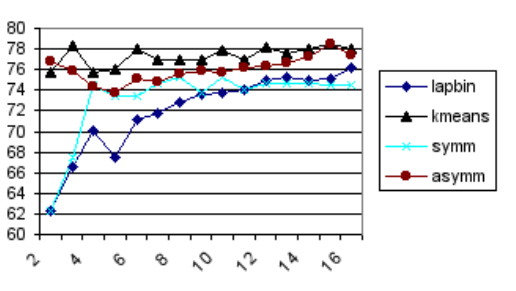
\includegraphics[scale=0.5]{clust.png}}}
 \caption{Comparison of different clustering algorithms with varying number of clusters and clustering accuracy}
 \label{fig:clust}
\end{figure}
	
	%%%%%%%%%%%%%%%%%%%%%%% F I G U R E %%%%%%%%%%%%%%%%%%%%%%%%%%%%
\begin{figure}
 \centerline{\framebox{
 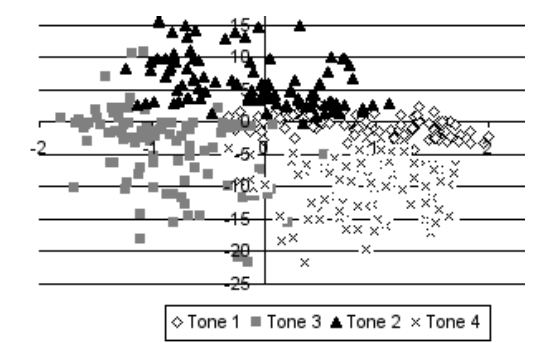
\includegraphics[scale=0.5]{heightslope.png}}}
 \caption{Cluster separation of pitch target slope (x) vs height (y) in Mandarin read speech data set}
 \label{fig:heightslope}
\end{figure}
	
	
\begin{comment}	
//time-series definition, representation, distance measure, algorithms, can be discussed in the time-series chapter,
if they occupy a special place in time-series research and is important. but it might not need to be in this
kind of chapter format, maybe could be more like lit review and not text book.

[new]
//general data mining?
6 unsupervised learning of tones
6.1 unsupervised learning
6.2 semi-supervised learning

%use this to discuss more on the literature, and specific to time-series mining, not general data mining.
%there is no special section on speech prosody mining. like lithuanian. but we can spread it in the
%discussion of the sub issues like distance computation.
%what about time-series tasks like exact motif search?
7. Time series mining of speech prosody
7.1 overview + basic definitions? + issues and applications like motif search
%normalization is here too

7.2 time-series representation
%mention speech representations and then discuss SAX

7.3 distance measures %techniques to speed up computation
     6.6.1 Euclidean distance . . . . . . . . . . . . . . . . . . . . 37
     6.6.2 DTW distance . . . . . . . . . . . . . . . . . . . . . . 37
     6.6.3 MINDIST distance function . . . . . . . . . . . . . . . 38
7.4 F0 pattern mining using time-series mining techniques	
\end{comment}
	
	
	%add the intonation based corpus research somewhere
	
	
\section{Speech prosody mining using time-series mining techniques}
Previous works in corpus based intonation research [Raskinis and Kazlauskiene 2013, Zhang 2015] have shown the challenges of data mining and clustering of speech intonation data in a large spoken / intonation corpus. At the core of this task is the expensive computation of a large amount of high-dimensional pairwise distance (especially with the widely preferred Dynamic Time Warping or DTW distance measure for time-series data) to obtain the distance matrix, and to find the most effective low-dimension feature representation for the F0 time-series data that faithfully preserve the true distances among objects with increased efficiency for storage.

[Zhang 2015] showed the potential of employing time-series data mining techniques to solve these problems, including techniques to speed up DTW distance computation [ ] and to transform feature representations for both dimensionality reduction and efficiency of computation and storage [ ]. In fact, F0 contour data can be naturally viewed as time-series data with F0 on the y-axis and time on the x-axis. Time-series mining has been successfully applied in a number of fields that deal with various kinds of time-series, including (the most relevant for our current purposes) Music Information Retrieval (MIR), where F0 contour data from music signal are indexed and searched, and meaningful patterns discovered [ ]. 

%where to put my specific results? 
%first read lin's review and sankalp paper again. and Keogh.



\subsection{Overview of time-series mining}
%ts mining introduction
%time series data mining
Formally, a time series T = $t_1$,...,$t_p$ is an ordered set of p real-valued variables, where $t_i$ is the time index. Time-series mining deals specifically with the data mining tasks with time-series data. [Lin et al 2007] outlined the main tasks that time-series mining research is concerned with:

(1) Indexing: Given a query time series Q, and some similarity/dissimilarity measure D(Q,C), find the most similar time series in database DB [2, 11, 20, 30, 63].

(2) Clustering: Find natural groupings of the time series in database DB under some similarity/dissimilarity measure D(Q,C) [29, 36].

(3) Classification: Given an unlabeled time series Q, assign it to one of two or more predefined classes [24].

(4) Summarization: Given a time series Q containing n datapoints where n is an extremely large number, create a (possibly graphic) approximation of Q which retains its essential features but fits on a single page, computer screen, executive summary etc [43].

(5) Anomaly Detection: Given a time series Q, and some model of �normal� behavior, find all sections of Q which contain anomalies or �surprising/interesting/unexpected/novel� behavior [14, 34, 54].

Due to the typical large size of data mining tasks and the high dimensionality of time-series, a generic time-series mining framework is as follows: [20] (1)Create an \textit{approximation} of the data, which will fit in main memory, yet retains the essential features of interest; (2) Approximately solve the task at hand in main
memory; (3)Make (hopefully very few) accesses to the original data on disk to confirm the solution obtained in Step 2, or to modify the solution so it agrees with the solution we would have obtained on the original data.

However, in practice, as will be discussed below, the success of this generic framework depends on the efficient time-series representation and distance measure in the approximated space that allows the lower bounding of true distances in the original space. The distance measure also needs to effectively capture the true (and meaningful) distances among objects, that also allows reasonably efficient computation (tractable) often by using special techniques to prune off impossible candidates. In the next sections I discuss some of the most relevant key issues in these areas.











%%%%%%%%%%%%%%%%%%%%%%%%%%%%% C O M M E N T S
\begin{comment}
Some distance measure Dist(A,B) must be defined in order to determine the similarity between time series objects A and B.\cite{lin:10}

\textbf{Distance:} Dist is a function that has A and B as inputs and returns a nonnegative value R, which is said to be the distance from A to B. \cite{lin:10}

It is well known that in high dimensional data, the notion of distance is weakened and all distances tend to be equal. For this reason, various dimensionality reduction and feature extraction / selection techniques are developed \cite{tan:05}.

Following the convention in the literature, each time series is normalized to have a mean of zero and a standard deviation of one before calling the distance function, since it is well understood that in virtually all settings, it is meaningless to compare time series with different offsets and amplitudes \cite{tan:05}. However, [Zhang 2015] shows that this normalization strategy does not work effectively for speech tones with level contours, which calls for an alternative strategy for normalization.

\textbf{Distance measure:} A distance measure provides a metric of dissimilarities between objects, with certain properties. A distance measure that satisfies (1)positivity;(2)Symmetry;(3)Triangle Inequality properties is known as a distance metric.


In time-series data, in addition to the well known Euclidean distance, it is also common to apply distance measures that can non-linearly map points in a time series to another, therefore addressing objects that are time shifted but otherwise are similar (such as a pair of strings that are shifted by one letter, but otherwise are identical). In this study, we also use Dynamic Time Warping (DTW) distance measure (\figref{fig:dtw}), which is a non-linear distance measure.\footnote{DTW is strictly speaking not a distance metric since it does not satisfy the triangle inequality.}

\textbf{Feature / representation:} It is frequently possible to create, from the original attributes, a new set of attributes that captures the important information in a data set much more effectively, known as features. 

Due to the typical high dimensionality of time-series data, feature representation has become a key area of research in time-series data mining. While some of these representations are more universally applicable, in many tasks it is still the best practice to develop problem-specific representations that achieves the optimal results. [Zhang 2015] experimented with both numeric and symbolic based representations, some of which are developed specifically in the realm of tone modeling. \figref{fig:ts-rep} shows an overview of many types of time-series representations in literature (adapted from [Lin 2010]). 

\end{comment}
%%%%%%%%%%%%%%%%%%%%%%%%%%%%%%%%%%%%%%%%%%%%%%%




















\subsection{Time-series and $F_0$ feature representation}
In Section \ref{sec:prosodic}, I have reviewed prosodic models and their relevance to feature representation of F0 contours in speech. Meanwhile, a great number of representations have been proposed for time-series mining, including both real-valued (such as DFT, DWT) and symbolic representations (Such as SAX). \figref{fig:ts-rep} illustrates the most commonly used representations [Lin 2010 ].

In the next sections I consider both types of feature representations and discuss their strength and limitations.




  

%a figure
\begin{figure}
 \centerline{\framebox{
 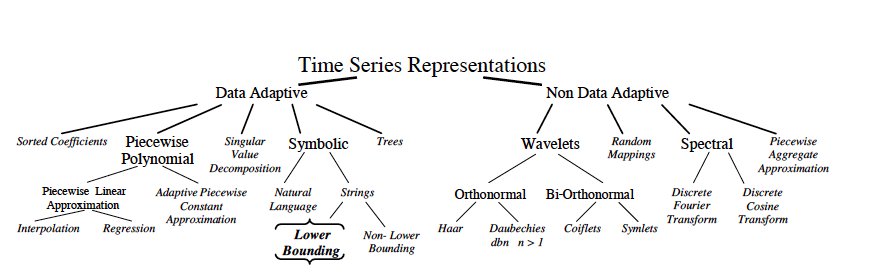
\includegraphics[scale=0.5]{ts-rep.png}}}
 \caption{Types of Time-series Data Representations (adapted from Lin 2010)}
 \label{fig:ts-rep}
\end{figure}

\subsubsection {Prosodic modeling feature representation}

%(1)numeric representation: qTA, polynomial fitting, raw F0 vector (diff or same length),D1

(1) \textbf{Polynomial Regression.} The most straightforward way to model F0 contour curves is to use polynomial functions to fit the F0 contour of each utterance. A F0 contour can thus be represented by the coefficient vector [$c_1$, $c_2$,..., $c_{n+1}$] of a \textit{n}-th order polynomial. This has been done in a number of studies for tone and intonation [ Hirst et al., 2000; Liu et al., 2006, and many others]. Alternatively, one could use a spline function, a piece-wise polynomial to model different sections of a complex contour. This approach greatly reduces the dimensionality of the original F0 contour.  However, [Xu 2011] points out that the critical question about polynomial representations is that whether they are linguistically meaningful, and whether they can be used in predictive modeling, i.e., serving as categorical parameters that can be generalized to other instances of the same category. This has not been evaluated in a predictive synthesis context. [Zhang 2015] experimented with the third degree polynomial representation (a 4d vector) of F0 contours in a clustering task with a clean read data set of Mandarin tones. The conclusion suggests that the clustering accuracy is low.
 
 


(2) \textbf{quantitative Target Approximation.} Given that qTA model (see section \ref{sec:qta}) has been shown to perform well in producing curves that closely resemble real tone contours in connected speech, an important question to be asked is: do qTA parameters perform well to reflect the similarities between tones in perception? In other words, we want to make sure that qTA parameters have the property where perceptually similar tone contour shapes also have similar parameter values. In [Zhang 2015]'s experiments the results suggest a negative answer to this question.


(3) \textbf{Raw Time-series F0 Vector}. [Gauthier et al 2007] showed that unsupervised classification using Self-Organizing Map (Neural Network) yielded a nearly 80\% correct result when time-series are represented with a 30-point raw F0 vector. 

In [Zhang 2015], in order to find the best method of working with F0 vectors, several transformations are made from the raw F0 vectors, including un-normalized and normalized. For each of these, in order to avoid the logarithmic behavior of Hertz unit, three versions are created, using Hertz, Bark, and Cent scale representations, giving rise to a total of 6 types of feature vectors. The conversion from Hertz to Bark and Cent are computed as below:

\begin{equation}
F_{CENT}=1200 * log_2 \frac{F_{HZ}}{F_{REF}}
\end{equation}

where the $F_{REF}$ is the reference frequency, corresponding to the minimum F0 in the computation of the pitch track (set to 55Hz).

\begin{equation}
F_{BK}=7*log [F_{HZ}/650 + ([1+(F_{HZ}650)^{2}]^{1/2})]
\end{equation}

In a series of clustering experiments, [Zhang 2015] found that (1) normalized contours yields higher accuracy than raw F0 contours; (2) the use of Hertz, Bark, or Cent scales did not have significant differences in the results; (3) the F0 vector achieves much higher accuracy with the DTW distance measure than Euclidean distance measure. 



(4) \textbf{First Derivative Vector (D1)}. The discrete first derivative feature (D1) is obtained simply by taking the first derivative of the original signal of the tone contour, and downsampled to 30 point:

\begin{equation}
D1=0.5 * (F_0 (t+1) - F_0(t-1))
\end{equation}

for all timestamps \textit{t}.

Intuitively, the D1 feature captures the movement of the pitch trajectory at each timestamp. It also serves as a normalization strategy where the differences in pitch height among different speakers are removed. Otherwise, the D1 does not reduce the dimensionality of the time series, nor does it create new abstract features as a combination of other features. As a first glance, it is not a fundamentally different transformation over the F0 feature. Surprisingly, [Gauthier et al 2007] showed a near-perfect performance using the D1 feature in a classification task with Self-Organizing Map. In the same experiment, the F0 feature performs around 20\% lower than the D1 feature. In [Zhang 2015], results suggest that D1 feature also achieves superior performance in unsupervised clustering tasks even when paired with Euclidean distance, in contrast to the F0 vector.










\subsubsection{Time-series symbolic representation}
[Lin et al 2007] points out the limitations in data mining algorithms for real-valued time-series representations (such as DFT and DWT). For example, in anomaly detection we cannot meaningfully define the probability of observing any particular set of wavelet coefficients, since the probability of observing any real number is zero [38]. Such limitations have led researchers to consider using a symbolic representation of time series.

There has been many symbolic representations proposed for time-series [3, 27]. However, none of the techniques allows a distance measure that lower bounds a distance measure defined on the original time series. This constitutes a problem for the generic time-series mining framework discussed above, since the approximate solution to problem created in main memory may be arbitrarily dissimilar to the true solution that would have been obtained on the original data. A symbolic approach that allows lower bounding of the true distance would not only satisfy the requirement of the generic framework, but also enables us to use a variety of algorithms and data structures which are only defined for discrete data, including hashing, Markov models, and suffix trees [Lin et al 2007] . Symbolic Aggregation approXmation (or SAX) [Lin 2010] is the first symbolic representation for time series that allows for dimensionality reduction and indexing with a lower-bounding distance measure at the same time. The related MINDIST distance function for SAX is discussed in Section \ref{sec:dist}.

 

The SAX representation transforms the pitch contour into a symbolic representation using Piecewise Aggregate Approximation technique (PAA, \figref{fig:paa}), with a user-designated length ($\textit{w}$=desired length of the feature vector) and alphabet size ($\textit{a}$), the latter being used to divide the pitch space of the contour into $\textit{a}$ equiprobable parts assuming a Gaussian distribution of F0 values (\figref{fig:sax}). Here, the Gaussian distribution is used to obtain the breakpoints for vertial pitch space so that each region (represented by a symbol) is equiprobable (probability of that symbol is given by the integration of the area under the Gaussian curve to as defined by the break points). This ensures that the probability of a segment being assigned any symbol is the same. \figref{fig:sax} shows an example [Lin et al 2007] of SAX transformation of a time-series of length 128. It is discretized by first obtaining a PAA approximation and then using predetermined breakpoints to map the PAA coefficients into SAX symbols. 



%SAX as used in MIR and by me
SAX has been evaluated in various classic time-series mining tasks and shown to work well in numerous applications to mine data from a variety of fields such as bioinfomatics, finance, telemedicine, audio and image signal processing, and network traffic analysis. In particular, it has been shown to preserve meaningful information from the original data and produce competitive results for classifying and clustering time series. 




%[Velaro ]
SAX has been less explored in the domain of audio signal F0 pattern mining. [Valero, Salamon and Gomez 2015] experimented with SAX representation for the computation of F0 contour similarity from music audio signals in a Query-By-Humming (QBH) task\footnote{In a query by humming task, a user hums a subsection of the melody of a desired song to search for the song from a database of music recordings.} in the context of Music Information Retrieval (MIR). However, results suggest that SAX does not perform well for musical time-series data in the context of QBH. The authors attribute this to the fact that SAX does not consider any particularities the origin domain of the time series may have - in this case, the musical notes. Thus, in the case of QBH, SAX may be abstracting away key musically-related information from the melodic contours required for properly performing the alignment [of F0 contour pairs]. 


%[zhang 2014,2015a,2015b]
[Zhang 2014, 2015a, 2015b] showed the effectiveness of SAX in mining speech or speech-like F0 contours - tones, where fine, noisy details of the F0 contours do not carry substantial crucial information comparing to its global shape. In [Zhang 2014], musical F0 contours from Beijing opera singing are converted to SAX representations in order to compare its similarity to linguistic tones of its lyrics. In a manually constructed data set consisted of balanced F0 contour shapes from all four tones, four types of evaluation measures showed that SAX representation faithfully preserves the original clusters. Similarly, [Zhang 2015b] experimented with the SAX parameters by iterating through different combinations of \textit{w} and \textit{a} to find the best correlation with the perceived pitch relationships in pairwise contour analysis. In [Zhang 2015a], SAX is shown to perform significantly better than raw F0-based contour features when subjected to the K-means clustering algorithm (see details in Section \ref{sec:speech mining}). This result is similar to the experiment on the Space Shuttle telemetry data set considered by [Lin et al 2003], where the SAX outperformed original data due to the possible smoothing effect of SAX's dimensionality reduction. In this context, contrary to the MIR melodic retrieval, the "abstracting" of SAX becomes a strength of the algorithm.




% distance measure, mindist, 


%%%%%%%%%%%%%%%%%%%%%%% F I G U R E %%%%%%%%%%%%%%%%%%%%%%%%%%%%
\begin{figure}
 \centerline{\framebox{
 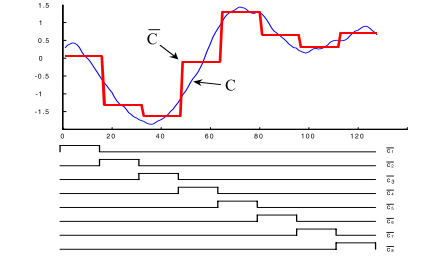
\includegraphics[scale=0.65]{paa.png}}}
 \caption{Piecewise Aggregate Approximation. The PAA representation can be visualized as an attempt to model a time series with a linear combination of box basis functions. In this case, a sequence of length 128 is reduced to 8 dimensions (adpated from [Lin et al 2007])}
 \label{fig:paa}
\end{figure}
%%%%%%%%%%%%%%%%%%%%%%%%%%%%%%%%%%%%%%%%%%%%%%%%%%


%%%%%%%%%%%%%%%%%%%%%%% F I G U R E %%%%%%%%%%%%%%%%%%%%%%%%%%%%
\begin{figure}
 \centerline{\framebox{
 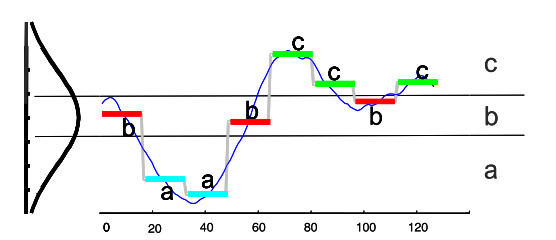
\includegraphics[scale=0.6]{sax.png}}}
 \caption{Symbolic Aggregate Approximation, with original length n = 128, number of segments w = 8 and alphabet size a = 3, with output word \textbf{baabccbc} (adpated from [Lin et al 2007])}
 \label{fig:sax}
\end{figure}
%%%%%%%%%%%%%%%%%%%%%%%%%%%%%%%%%%%%%%%%%%%%%%%%%%












\subsubsection{Time-series normalization}


%time-series normalization
Many literature reviews\cite{lin:10} in time-series mining assert that time series must be normalized using the z-score transformation normalization strategy so that each contour has a standard deviation of 1 and mean of 0 (in fact this is a general strategy that is also used in mining non-time-series data):

%z-score transformation formula
\begin{equation}
z=(x_i-\mu)/\sigma
\end{equation}

where $\mu$ is the mean of the contour and $\sigma$ is the standard deviation.

However, [Zhang 2015] observed that speech tone time-series data has a special property so that the z-score transformation would seriously distort the shapes of the tones in the normalized corpus. Essentially this is caused by the presence of many flat or near flat contours (such as in level tones). Since z-score transformation expresses each data point in a time series by its relative value to the mean in terms of standard deviation, it would magnify the differences in the values of the flat or near flat contours (since each point in this contour is identical and also identical to the mean), and turn such contours into a significantly un-flat contour. 

Since normalization is required for a meaningful comparison of time-series patterns, we need to design an alternative strategy for time-series normalization in this task. There are many strategies that fulfills this purpose. After trial and error experimentation, one of the best working measure is the Subtract-Mean normalization strategy (see Equation \ref{form-norm}). It effectively retains the original shapes in a normalized corpus of tones. 

%add equation

%z-score transformation formula
\begin{equation}
\label{form-norm}
z=(x_i-\mu)
\end{equation}


This issue also exists in SAX representation since normalized time-series SAX significantly outperforms un-normalized ones [Zhang 2015]. Therefore it is a built-in requirement of SAX to first normalize the time-series using z-score transformation. Fortunately, SAX also has a built-in remedy for this problem: when the standard deviation of a subsequence time-series is less than a pre-set threshold (a very small number), all of its segments will be assigned the same symbol. 



%Distance measure
\subsection{Distance measure} \label{sec:dist}
(1) \textbf{Euclidean distance}. The Euclidean distance is one the most widely used and computationally economic distance measures [Lin 2010], defined as follows on the \textit{n}-dimensional Euclidean space for a time-series of length \textit{n}:

\begin{equation}
d(p,q) = d(q,p) = \sqrt{\sum_{i=1}^{n} (q_i - p_i)^2} 
\end{equation}


(2) \textbf{DTW distance}. In time series analysis, dynamic time warping (DTW) is an algorithm for measuring similarity between two temporal sequences which may vary in time or speed (\figref{fig:dtw}). DTW distance between two time series is computed with dynamic programming, by recursively solving the optimal alignment between two sequences in subproblems, and return the shortest distance between the two (i.e., best alignment) time series. In particular, the optimal path is the path that minimizes the warping cost:

\begin{equation}
DTW(Q,C)=min\bigg\{\sqrt{\sum_{k=1}^{K} (w_k)}
\end{equation}

where $w_k$ is the matrix element $(i,j)_k$ that also belongs to k-th element of a warping path W, a contiguous set of matrix elements that represent a mapping between Q and C.

This warping path can be found using standard dynamic programming to evaluate the following recurrence.


\begin{equation}
\gamma (i, j) = d(q_i, c_j) + min\bigg\{\gamma(i-1,j-1), \gamma(i-1, j), \gamma(i,j-1)\bigg\}
\end{equation}

where d(i,j) is the distance found in the current cell, and $\gamma$(i,j) is the cumulative distance of d(i,j) and the minimum cumulative distances from the three adjacent cells.


To make the computation tractable and to prevent pathological warping, many constraints have been proposed to impose upon the possible warping window. One such window is shown in green in \figref{fig:dtw}. 


%a figure
\begin{figure}
 \centerline{\framebox{
 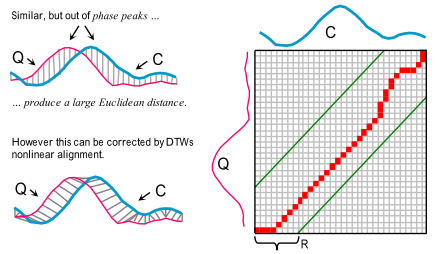
\includegraphics[scale=0.7]{dtw.png}}}
 \caption{Euclidean distance vs. Dynamic Time Warping: example (adapted from [Rakthanmanon et al 2012])}
 \label{fig:dtw}
\end{figure}


In practice, since DTW has a time complexity of \textit{O($n^2$)}, where \textit{n} is the length of the time-series, various lower-bounding techniques are proposed to speed up DTW distance computation in a large database. The LB\_Keogh lower bounding technique [Keogh et al 2004], for example, speeds up the computation by first taking an approximated distance between the time-series that is both fast to compute and lower bounds the true distance. It would go on to compute the real DTW distance only if this distance turns out to be smaller than the best-so-far, since there is no way in this case that the true distance is even smaller than the best so far. This makes DTW essentially an \textit{O($n$)} algorithm as we rarely have to do a full DTW calculation. The general approach is illustrated in \figref{fig:lbk}. This approach can be used in many applications that require DTW, such as exact motif search (see below discussion) and k-means clustering, where for each data point one needs to find its closest centroid. 


%a figure
\begin{figure}
 \centerline{\framebox{
 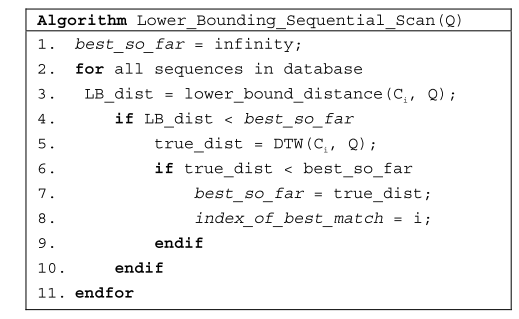
\includegraphics[scale=0.6]{lbk.png}}}
 \caption{An algorithm that uses a lower bounding distance measure to speed up the sequential scan search for the query Q (adapted from [Ratanamahata et al 2012])}
 \label{fig:lbk}
\end{figure}



(3) \textbf{MINDIST distance function. }The MINDIST function is a distance measure defined for the SAX representation of the time series, which, crucially, have been proved to lower bound the true distances of original data [Lin et al 2003]. It returns the minimum distance computed between two strings by building on the PAA representation distance function and substitute the distance computation with a subroutine of \texttt{dist()} function:




\begin{equation}
MINDIST(Q,C)= \sqrt{\frac{n}{w}} \sqrt{\sum_{i=1}^{w} dist(q_i , c_i)^2} 
\end{equation}

The \texttt{dist()} function can be implemented by search over a lookup table (for details see [Lin et al 2003]). The lower bounding property is an important heuristic for pruning sub-optimal candidate when finding the minimum distance: to avoid expensive computational cost of computing the true distances over a large number of time series, we can first use a SAX approximation to the original time series and compute the MINDIST distance matrix. Since the MINDIST is proved to lower bound the true distance, then we can prune off those whose MINDIST distance is greater than the best so far, since there is no way its true distance would be less than the best minimum distance so far. 













\begin{comment}


%%%%%%%%%%%%%% clustering algos

%Organization: try to do this by distance based (discriminative?) vs. generative models

\subsection{Unsupervised learning algorithms}
\subsubsection{Kmeans clustering}
% kmeans
The most commonly used clustering algorithm is k-means\cite{lin:10}. Originally developed as a technique of vector quantization in signal processing, k-means clustering aims to partition n observations into k clusters in which each observation belongs to the cluster with the nearest mean, serving as a prototype of the cluster. In this paper, we perform kmeans clustering as a basic evaluation strategy for the comparison of the accuracy of the clustering using feature \textit{f}. The accuracy measure is defined by comparing the assigned cluster labels to the true tone labels of each time series, obtaining a confusion matrix showing the true labels against the predicted labels of the cluster assignments, where predicted labels is the most predominant label (i.e., the tone category with the most number of instances among all tones assigned that label) within that cluster. The accuracy value of each clustering experiment is given along with the range of confidence intervals of that value. In this study we use the generic \texttt{kmeans} function for clustering numeric data (including any feature that has numeric values, dimensionality reduced or not) in \texttt{R}, and we use the \texttt{flexclust} package to perform k-means clustering on the SAX symbolic data using the pre-defined distance measure called \texttt{mindist}. The \texttt{mindist} distance matrix is computed with the \texttt{diss.MINDIST.SAX} function in the \texttt{TSClust} package in R.

% hierarchical - mainly used to evaluate SAX representation
\subsubsection{Hierarchical clustering}
One of the most widely used clustering approaches is hierarchical clustering [11]. Hierarchical clustering computes pairwise distances of the objects (or groups of objects) and produces a nested hierarchy of the clusters. It has several advantages over other clustering methods. More specifically, it offers great visualization power with the hierarchy of clusters, and it requires no input parameters. However, its intensive computational complexity makes it infeasible for large datasets\cite{lin:10}.

Even though hierarchical clustering gives an effective overview of the similarities between different levels of clusters, it is difficult to precisely compare results of clustering by looking at the dendrogram (as it is not straightforward to compute accuracy measures as in kmeans clustering). For this reason, in this study I only experiment with hierarchical clustering with in exploratory data analysis. Hierarchical clustering also serves as an evaluation for the SAX representation, as discussed later.

%validation of sax representation hinted



% model based clust
\subsubsection{Model based clustering}
In this experiment, model based clustering is performed with the \texttt{mclust} package (Normal Mixture Modeling for Model-Based Clustering, Classification, and Density Estimation) in \texttt{R}, using the Bayesian Information Criterion(BIC) as model selection criterion. The clustering experiments (both in model based and kmeans clustering) are done with two parameter settings: first, we perform clustering with a range of parameters G=1:9, letting the algorithm select the best number of clusters using BIC; Next, we perform clustering with number of cluster = 4 specified. This method models the clusters as multivariate Gaussians, therefore is particularly indicative of the Gaussian property of the tone categories.
\end{comment}













\subsection{F0 pattern mining using time-series mining techniques} \label{sec:speech mining}

%lets talk about the applications and possible tasks for this area. example: 
[Ratanamahatana et al 2004] shows that there are many data mining tasks that can be more efficiently solved as a time-series mining task, including video / image / handwriting retrieval, and text mining. In this section I discuss previous work that is closely related to F0 pattern mining (as in the current proposed project), including music information retrieval F0 melodic pattern mining, and speech intonation mining.

[Gulati et al 2014] applied exact motif (pattern) discovery to the F0 melodic patterns large collection of Indian music recordings by computing similarity between every possible subsequence pair obtained within an audio recording. This works exemplifies an integration of a variety of time-series mining techniques applied in different tasks crucial for F0 pattern mining in music (and in many cases, in speech) melodic pattern discovery, including distance measures, time-series representation, exact motif discovery[ ], lower bounding in DTW distance computation [ ] and early abandoning in exact motif discovery [  ]. 



%what is exact motif search?
Discovery of repeating structures in F0 contours is fundamental to the analysis, understanding and interpretation of its intrinsic structure in both speech and music. At the center of this study is the motif discovery task in time-series. Time series motifs are pairs of individual time series, or subsequences of a longer time series, which are very similar to each other. Therefore, the task of motif discovery is to find all pairs or groups of highly similar subsequences or individual time-series in a large collection of time series data, in an \textit{unsupervised} manner.  Because the obvious algorithm for computing motifs is quadratic in the number of items, more than a dozen \textit{approximate} algorithms to discover motifs have been proposed in the literature. [Mueen et al 2009] proposed the first tractable \textit{exact} motif discovery algorithm that is up to three orders of magnitudes faster than the brute force search algorithm. This is done through a combination of early pruning strategies and early abandoning of distance computation once the computed distance exceeds the best-so-far. 




In [Gulati et al 2014], intra-recording pattern discovery is performed first through this state-of-the-art exact motif discovery algorithm. Top k pairs of motifs known as 'seed' patterns are stored for further evaluation. Subsequently the algorithm searches for their repetitions in the entire music collection. Similarity between melodic patterns are computed using dynamic time warping (DTW), where four different variants of the DTW cost function for rank refinement of the obtained results are evaluated. Over 13 trillion DTW distance computations are done for the entire dataset (360+ hours of music recordings). Due to the computational complexity of the task, different lower bounding and early abandoning techniques are applied during DTW distance computation. An evaluation based on expert feedback on a subset of the dataset shows that the discovered melodic patterns are musically relevant. Several musically interesting relationships are discovered, yielding further scope for establishing novel similarity measures based on melodic patterns. As an outcome of this work, Gulati et al. developed an interactive search tool where users can query and search for the top k similar melodic patterns, which can be further inspected (audio) and analyzed [ ]. \figref{fig:netvis} shows a network visualization of the global and individual patterns found through through unsupervised learning, which allows users to interactively zoom in and out to explore the similarity structure at different levels [ ].  

%show the possible applications of the search tool and network visualization.



%%%%%%%%%%%%%%%%%%%%%%% F I G U R E %%%%%%%%%%%%%%%%%%%%%%%%%%%%
\begin{figure}
 \centerline{\framebox{
 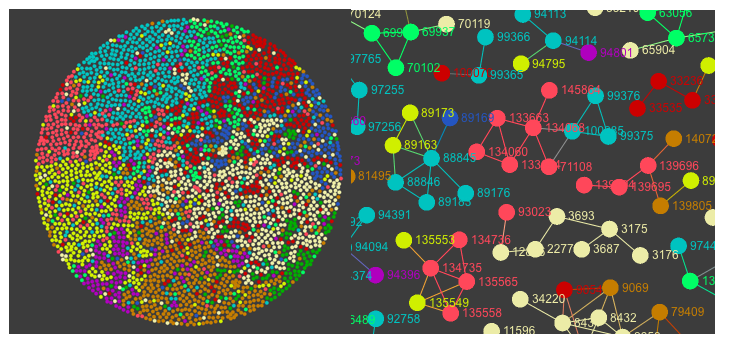
\includegraphics[scale=0.5]{sankalp.png}}}
 \caption{Network visualization of melodic patterns mined from a large collection of Indian music. Left: Global structure. Right: Individual similarity groupings. Each node represents a subsequence (pattern) of melodic contours about 2s long. }
 \label{fig:netvis}
\end{figure}
%%%%%%%%%%%%%%%%%%%%%%%%%%%%%%%%%%%%%%%%%%%%%%%%%%


%Sankalp 2015
As mentioned above, one of the most important aspect of F0 time-series pattern mining is the choices made for time-series representation, normalization techniques and distance measures. [Gulati et al 2015] performed a comparative evaluation of methodologies for computing similarity between short-time melodic fragments of audio recordings of Indian art music. Gulati et al. experiment with 560 different combinations of procedures and parameter values, including sampling rate of the melody representation, pitch quantization levels, normalization techniques and distance measures. The results indicate that melodic fragment similarity is particularly sensitive to distance measures and normalization techniques, while sampling rate plays a less important role. Furthermore, the author claims that this type of work paves the way for developing unsupervised melodic pattern discovery approaches, whose evaluation is a challenging and, many times, ill-defined task. Both of these issues (the parameters and the definition of the evaluation of the task) are related to similar task in speech F0 pattern mining. 


%zhang 2015
[Zhang 2015a] investigated the use of time-series mining techniques in the unsupervised learning of Mandarin tones using a read speech data set from [Xu 1997]. In this work, various types of time-series representation, distance measures, and normalization procedures are evaluated with k-means clustering algorithm to find the most effective parameters for tone learning. The result suggests that (1) The D1 (first derivative) feature significantly outperforms the F0-based features when paired with Euclidean distance. (2) The LB\_Keogh lower bounding technique significantly speeds up the computation of DTW distance, which obtained superior results even with F0-based features; (3) SAX feature is a low-dimension yet effective feature that obtains the same level of performance as the D1 feature (with MINDIST distance measure); (4) polynomial and qTA model coefficient based features perform below chance in this task. These behaviors of different features and distance measures with regard to the k-means clustering algorithm is shown in \figref{fig:kmof}. In particular, the polynomial and qTA parameters show periodic oscillation of k-means objective function (intra-cluster distances), without a trend to converge. The distance matrix in \figref{fig:saxhc} and \figref{fig:edhc} may give a hint as to why SAX outperforms the F0 features with Euclidean distance: In \figref{fig:saxhc} we can clearly see that the lower dimension SAX-MINDIST distance reflects the intrinsic structure of the clusters with lower distance along the diagonal (from top left to bottom right); However, in \figref{fig:edhc}, which uses 30-dimension F0 contour feature, the distances are all somewhat equalized. 




%%%%%%%%%%%%%%%%%%%%%%% F I G U R E %%%%%%%%%%%%%%%%%%%%%%%%%%%%
\begin{figure}
 \centerline{\framebox{
 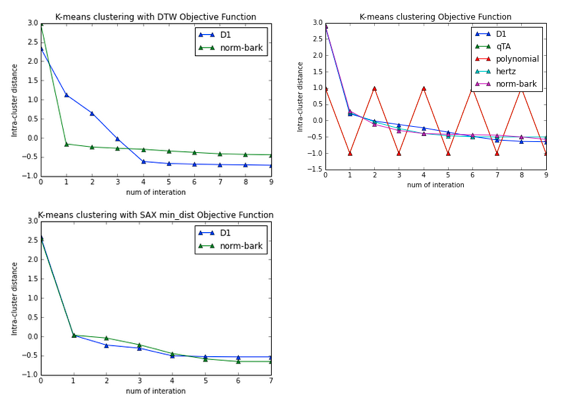
\includegraphics[scale=0.7]{kmeansOF.png}}}
 \caption{Kmeans clustering objective function by number of iteration. Intra-cluster distance (y axis) is normalized. "norm-bark" is normalized Bark scale of F0 values. The top plots show numeric representations of time-series with DTW and Euclidean distance. The bottom plot shows the SAX representation with MINDIST distance. }
 \label{fig:kmof}
\end{figure}
%%%%%%%%%%%%%%%%%%%%%%%%%%%%%%%%%%%%%%%%%%%%%%%%%%




%%%%%%%%%%%%%%%%%%%%%%% F I G U R E %%%%%%%%%%%%%%%%%%%%%%%%%%%%
\begin{figure}
 \centerline{\framebox{
 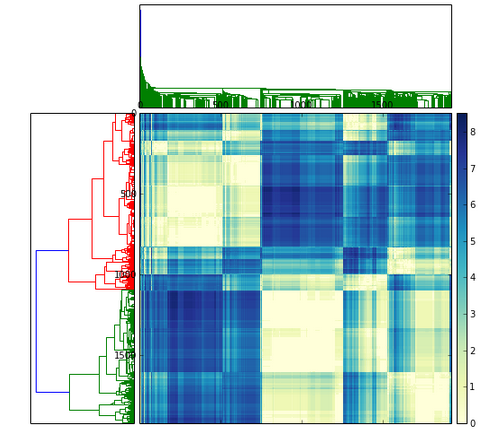
\includegraphics[scale=0.5]{distsax.png}}}
 \caption{SAX-MINDIST Distance matrix of 1600 Mandarin tones sorted by tone category. Top and Left show the hierarchical clustering of tones using single-linkage and centroid distance}
 \label{fig:saxhc}
\end{figure}
%%%%%%%%%%%%%%%%%%%%%%%%%%%%%%%%%%%%%%%%%%%%%%%%%%


%%%%%%%%%%%%%%%%%%%%%%% F I G U R E %%%%%%%%%%%%%%%%%%%%%%%%%%%%
\begin{figure}
 \centerline{\framebox{
 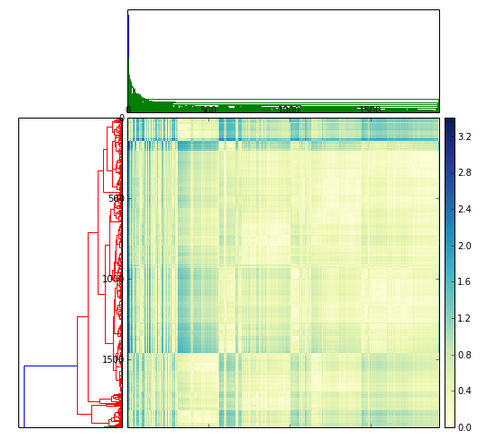
\includegraphics[scale=0.5]{disted.png}}}
 \caption{F0-Euclidean Distance matrix of 1600 Mandarin tones sorted by tone category. Top and Left show the hierarchical clustering of tones using single-linkage and centroid distance}
 \label{fig:edhc}
\end{figure}
%%%%%%%%%%%%%%%%%%%%%%%%%%%%%%%%%%%%%%%%%%%%%%%%%%


%include the accuracy result table. 


%\section{Prosody based dialect detection via unsupervised learning}
\section{ Chapter outlines}





\end{document}
